\chapter[Tensor decomposition]{Discussion about the Tensor decomposition within the HiDeNN framework}
\label{chap:TD}
\begin{chapabstract}
    This chapter investigates the link between the HiDeNN framework and the classical tensor decomposition used in standard Reduced-order modelling (ROM) techniques.
\end{chapabstract}

\minitoc
\section{Reduced-Order modelling (ROM)}

    Reduced-order modelling methods offer a way to escape the curse of dimensionality. The idea is to express it as a sum of products of single variable functions. Let's consider a displacement field $\vect{u}$ parameterised by the position $\vect{x}$ and a set of $\beta$ parameters $\left\{\mu_i\right\}_{i \in \llbracket 1, \beta \rrbracket}$. Its reduced-order expression using $m$ modes reads
    \begin{equation}
        \vect{u}\left(\textcolor{BleuLMS!70}{\vect{x}}, \textcolor{LGreenLMS}{\left\{\mu_i\right\}_{i \in \llbracket 1, \beta \rrbracket}}\right) = \sum\limits_{i=1}^m \textcolor{BleuLMS!70}{\overline{\vect{u}}_i(\vect{x})} ~\textcolor{LGreenLMS}{\prod_{j=1}^{\beta}\lambda_i^j(\mu^j)}.
    \end{equation}

\section{HiDeNN-ROM}



The aforementioned tensor decomposition can be used in the HiDeNN framework \parencite{zhang_hidenn-td_2022} using the \emph{Multiplication block} $\mathcal{M}$ detailed in \parencite{zhang_hierarchical_2021}. Such an implementation falls in the scope of \emph{a priori} reduced-order modelling \parencite{ryckelynck_thea_2006,chinesta_short_2011} as no prior knowledge is required (those methods do not require offline expensive computations to build the reduced-order basis).

\subsection{Single parameter}
\begin{wrapfigure}{r}{0.45\textwidth}
\vspace{-65pt}
    \flushleft
    % \tikzsetnextfilename{NN_TD}
    \tikzstyle{input} = [circle, draw=BleuLMS, fill=BleuLMS!25, minimum size=8mm, thick]

\tikzstyle{inputSpace} = [circle, circular drop shadow, draw=GreenLMS, fill=BleuLMS!25, minimum size=8mm, thick]
\tikzstyle{inputPara} = [circle, circular drop shadow, draw=LGreenLMS, fill=LGreenLMS!25, minimum size=8mm, thick]

\tikzstyle{ShapeF} = [circle, draw=GreenLMS, fill=GreenLMS!25, minimum size=2mm, thick]

\tikzstyle{Sol} = [circle, circular drop shadow, draw=LGreenLMS, fill=LGreenLMS!25, minimum size=2mm, thick]
\tikzstyle{Out} = [circle, circular drop shadow, draw=BleuLMS, fill=GreenLMS!25, minimum size=2mm, thick]
\tikzstyle{Mul} = [circle, circular drop shadow, draw=black, fill=black!25, minimum size=2mm, thick]
\tikzstyle{lineSpace} = [draw,BleuLMS, -,thick]
\tikzstyle{linePara} = [draw,LGreenLMS, -,thick]
\tikzstyle{line} = [draw,GreenLMS, -,thick]
\tikzstyle{lineDot} = [draw,GreenLMS, doted,thick]
\usetikzlibrary {math}
\usetikzlibrary {decorations}
\usetikzlibrary{shadows}



	\begin{tikzpicture}[>=Stealth, node distance=1.5cm]

		\def\NN{4} % number of nodes in spatial mesh
		\def\NU{3} % number of nodes in parameter mesh
		\def\NM{2} % number of modes
		

		
		% Input layer
		\foreach \i in {1}
		\node [inputSpace] (I\i) at (0,-1.5-2.5) {$x$};
		
		\foreach \i in {2}
		\node [inputPara] (I\i) at (0,-1-1.5-6.5) {$\mu$};
		
		% Hidden layer
		\foreach \h [count=\hi] in {1,...,\NN}
		\node [inputSpace] (Ho\hi) at (2, -1.1*\h) {$N^{\Omega}_\h$};
		\node [inputSpace] (Last) at (2, -1.1*\NN-1.5) {$N^{\Omega}_p$};
		\draw[dotted, very thick,GreenLMS ] (Ho\NN) -- (Last);
	
		\foreach \h [count=\hi] in {1,...,\NU}
		\node [inputPara] (Hm\hi) at (2, -1.5-4.5-1.1*\h) {$N^{\mu}_\h$};
		\node [inputPara] (Last2) at (2, -1.5-4.5-1.1*\NU-1.5) {$N^{\mu}_q$};
		\draw[ dotted, very thick, LGreenLMS] (Hm\NU) -- (Last2);
		
		% 2nd hidden layer
		\foreach \o [count=\oi] in {1,...,\NM}
		\node [inputSpace] (O\oi) at (4, -1-1.3*\oi) {$\overline{u}_\o(x)$};
		\node [inputSpace] (OLast) at (4, -1-1.3*\NM-1.7) {$\overline{u}_m(x)$};
		\draw[dotted, very thick,GreenLMS ] (O\NM) -- (OLast);
		
		\foreach \o [count=\oi] in {1,...,\NM}
		\node [inputPara] (Om\oi) at (4, -1.5-5-1.3*\oi) {$\lambda_\o(\mu)$};
		\node [inputPara] (OLastm) at (4, -1.5-5-1.3*\NM-1.7) {$\lambda_m(\mu)$};
		\draw[dotted, very thick,LGreenLMS ] (Om\NM) -- (OLastm);
		
		% 3rd hidden layer
		
		\foreach \o [count=\oi] in {1,...,\NM}
		\node [Mul] (Mul\oi) at (6, -1.5-3-\oi) {$\mathcal{M}$};
		\node [Mul] (MulLast) at (6, -1.5-3-\NM-1.5) {$\mathcal{M}$};
		\draw[dotted, very thick,black ] (Mul\NM) -- (MulLast);
		
		%		 output layer
				\node [Out] (Iout) at (8,-1.5-4.5) {$u\left(x,\mu\right)$};
		
		% Connect layers
		\foreach \i in {1}
		\foreach \h in {1,...,\NN}
		\draw [lineSpace] (I\i) -- (Ho\h);
		
		\draw [lineSpace] (I1) -- (Last);
		\draw [linePara] (I2) -- (Last2);
		
		\foreach \i in {2}
		\foreach \h in {1,...,\NU}
		\draw [linePara] (I\i) -- (Hm\h);
		
		\foreach \h in {1,...,\NN}
		\foreach \o in {1,...,\NM}
		\draw [lineSpace] (Ho\h) -- (O\o);
		
		\draw [lineSpace] (Last) -- (O\NM);
		
		\foreach \h in {1,...,\NN}
		\draw [lineSpace] (Ho\h) -- (OLast);
		
		\foreach \h in {1,...,\NM}
		\draw [lineSpace] (Last) -- (O\h);
		
		\draw [lineSpace] (Last) -- (OLast);
		
		\foreach \h in {1,...,\NU}
		\foreach \o in {1,...,\NM}
		\draw [linePara] (Hm\h) -- (Om\o);
		
		\foreach \h in {1,...,\NU}
		\draw [linePara] (Hm\h) -- (OLastm);
		\foreach \h in {1,...,\NM}
		\draw [linePara] (Last2) -- (Om\h);
		
		\draw [linePara] (Last2) -- (OLastm);
		

		\foreach \m in {1,...,\NM}
		\draw [lineSpace] (O\m) -- (Mul\m);
		\foreach \m in {1,...,\NM}
		\draw [linePara] (Om\m) -- (Mul\m);
		
		\draw [lineSpace] (OLast) -- (MulLast);
		\draw [linePara] (OLastm) -- (MulLast);

		
				\foreach \m in {1,...,\NM}
		\draw [line] (Mul\m) -- (Iout);
		
		\draw [line] (MulLast) -- (Iout);
		
%		% Layer labels
%		\node[above=of I1] {Input Layer};
%		\node[above=of Ho1] {Hidden Layer};
%		\node[above=of O1] {Output Layer};
	\end{tikzpicture}
    \caption{HiDeNN-TD for a single extra parameter}
    \label{fig:HiDeNN_TD_mu}
\end{wrapfigure}
The HiDeNN framework consists of an interpolation network based, for instance, on the finite element shape functions $N$. Let us consider the following tensor decomposition.
\begin{equation}
    \vect{u}(\textcolor{BleuLMS!70}{\vect{x}},\textcolor{LGreenLMS}{\mu}) = \sum\limits_{i=1}^m \textcolor{BleuLMS!70}{\overline{\vect{u}}_i(\vect{x})} ~\textcolor{LGreenLMS}{\lambda_i(\mu)}
\end{equation}
The HiDeNN architecture leading to such a decomposition of the interpolation is illustrated in Figure~\ref{fig:HiDeNN_TD_mu}. The \textcolor{BleuLMS!70}{blue Neural Network} allows the interpolation of the spatial modes using given finite element shape functions. The \textcolor{LGreenLMS}{green Neural Network} would probably only use 1D shape functions to interpolate scalar parameter fields. For each $i \in \llbracket 1, m \rrbracket$ mode, both element of the pair $\left(\textcolor{BleuLMS!70}{\vect{\overline{u}}_i}, \textcolor{LGreenLMS}{\lambda_i} \right)$ are multiplied with each others. the last layer sums all the products of the tensor decomposition. 
The loss function can later be computed using the input parameters and the output interpolation. An optimiser is then used to train the NN, \emph{i.e.} solve the optimisation problem. 

Note: The top part of the NN up to $\vect{\overline{u}}_1\left(x\right)$ corresponds to a classical quasi-static HiDeNN. 

\Rqs{There are (as classically in ROM) $\left(p+q\right)\times m$ unknowns $+\left(p+q\right)$ additional unknowns for the nodal coordinates}{The classical \emph{Update stage} of the PGD can be achieved by freezing the $\left\{u_i\right\}_{i \in \llbracket 1,m \rrbracket}$.}
\begin{figure}
    \flushright
        % \tikzsetnextfilename{HiDeNN_MultiP}
    \tikzstyle{input} = [circle, draw=BleuLMS, fill=BleuLMS!25, minimum size=8mm, thick]

\tikzstyle{inputSpace} = [circle, circular drop shadow, draw=GreenLMS, fill=BleuLMS!25, minimum size=8mm, thick]
\tikzstyle{inputPara} = [circle, circular drop shadow, draw=LGreenLMS, fill=LGreenLMS!25, minimum size=8mm, thick]

\tikzstyle{ShapeF} = [circle, draw=GreenLMS, fill=GreenLMS!25, minimum size=2mm, thick]

\tikzstyle{Sol} = [circle, circular drop shadow, draw=LGreenLMS, fill=LGreenLMS!25, minimum size=2mm, thick]
\tikzstyle{Out} = [circle, circular drop shadow, draw=BleuLMS, fill=GreenLMS!25, minimum size=2mm, thick]
\tikzstyle{Mul} = [circle, circular drop shadow, draw=black, fill=black!25, minimum size=2mm, thick]
\tikzstyle{lineSpace} = [draw,BleuLMS, -,thick]
\tikzstyle{linePara} = [draw,LGreenLMS, -,thick]
\tikzstyle{line} = [draw,GreenLMS, -,thick]
\tikzstyle{lineDot} = [draw,GreenLMS, doted,thick]
\usetikzlibrary {math}
\usetikzlibrary {decorations}
\usetikzlibrary{shadows}



		\begin{tikzpicture}[>=Stealth, node distance=1.5cm]
		
		\def\NN{4} % number of nodes in spatial mesh
		\def\NU{3} % number of nodes in parameter mesh
		\def\NM{2} % number of modes
		
		
		
		% Input layer
		\foreach \i in {1}
		\node [inputSpace] (I\i) at (0,-1.5-2.5) {$x$};
		
		\foreach \i in {2}
		\node [inputPara] (I\i) at (0,-1-1.5-6.5) {$\mu^1$};
		
		\foreach \i in {3}
		\node [inputPara] (I\i) at (0,-6-1-1.5-6.5) {$\mu^{\beta}$};
		
		\foreach \i in {2}
		\foreach \h in {3}
		\draw[loosely dotted, very thick,LGreenLMS] (I\i) -- (I\h);
		
		%% Hidden layer
		\foreach \h [count=\hi] in {1,...,\NN}
		\node [inputSpace] (Ho\hi) at (2, -1.1*\h) {$N^{\Omega}_\h$};
		\node [inputSpace] (Last) at (2, -1.1*\NN-1.5) {$N^{\Omega}_p$};
		\draw[dotted, very thick,GreenLMS ] (Ho\NN) -- (Last);
		
		\foreach \h [count=\hi] in {1,...,\NU}
		\node [inputPara] (Hm\hi) at (2, -1.5-4.5-1.1*\h) {$N^{\mu}_\h$};
		\node [inputPara] (Last2) at (2, -1.5-4.5-1.1*\NU-1.5) {$N^{\mu}_q$};
		\draw[ dotted, very thick, LGreenLMS] (Hm\NU) -- (Last2);
		
				% Last parameter
				\foreach \h [count=\hi] in {1,...,\NU}
				\node [inputPara] (Hmbeta\hi) at (2, -6-1.5-4.5-1.1*\h) {$N^{\mu}_\h$};
				\node [inputPara] (Last2beta) at (2, -6-1.5-4.5-1.1*\NU-1.5) {$N^{\mu}_q$};
				\draw[ dotted, very thick, LGreenLMS] (Hmbeta\NU) -- (Last2beta);
		
		% 2nd hidden layer
		\foreach \o [count=\oi] in {1,...,\NM}
		\node [inputSpace] (O\oi) at (4, -1-1.3*\oi) {$\overline{u}_\o(x)$};
		\node [inputSpace] (OLast) at (4, -1-1.3*\NM-1.7) {$\overline{u}_m(x)$};
		\draw[dotted, very thick,GreenLMS ] (O\NM) -- (OLast);
		
		\foreach \o [count=\oi] in {1,...,\NM}
		\node [inputPara] (Om\oi) at (4, -1.5-5-1.3*\oi) {$\lambda_\o^1(\mu)$};
		\node [inputPara] (OLastm) at (4, -1.5-5-1.3*\NM-1.7) {$\lambda_m(\mu)$};
		\draw[dotted, very thick,LGreenLMS ] (Om\NM) -- (OLastm);
				% Last parameter
					\foreach \o [count=\oi] in {1,...,\NM}
					\node [inputPara] (Ombeta\oi) at (4, -6-1.5-5-1.3*\oi) {$\lambda_\o^{\beta}(\mu)$};
					\node [inputPara] (OLastmbeta) at (4, -6-1.5-5-1.3*\NM-1.7) {$\lambda_m^{\beta}(\mu)$};
					\draw[dotted, very thick,LGreenLMS ] (Ombeta\NM) -- (OLastmbeta);
		
		% 3rd hidden layer
		
		\foreach \o [count=\oi] in {1,...,\NM}
		\node [Mul] (Mul\oi) at (7, -2.5-1.5-3-\oi) {$\mathcal{M}$};
		\node [Mul] (MulLast) at (7, -2.5-1.5-3-\NM-1.5) {$\mathcal{M}$};
		\draw[dotted, very thick,black ] (Mul\NM) -- (MulLast);
		
		%		 output layer
		\node [Out] (Iout) at (9,-2.5-1.5-4.5) {$u\left(x,\mu\right)$};
		
		% Connect layers
		\foreach \i in {1}
		\foreach \h in {1,...,\NN}
		\draw [lineSpace] (I\i) -- (Ho\h);
		
			\draw [lineSpace] (I1) -- (Last);
			\draw [linePara] (I2) -- (Last2);
			\draw [linePara] (I3) -- (Last2beta);
		
		\foreach \i in {2}
		\foreach \h in {1,...,\NU}
		\draw [linePara] (I\i) -- (Hm\h);
		
	
		
		
			\foreach \i in {3}
			\foreach \h in {1,...,\NU}
			\draw [linePara] (I\i) -- (Hmbeta\h);
		
		\foreach \h in {1,...,\NN}
		\foreach \o in {1,...,\NM}
		\draw [lineSpace] (Ho\h) -- (O\o);
		\draw [lineSpace] (Last) -- (O\NM);
		
		\foreach \h in {1,...,\NN}
		\draw [lineSpace] (Ho\h) -- (OLast);
		\draw [lineSpace] (Last) -- (OLast);
		
		\foreach \h in {1,...,\NM}
		\draw [lineSpace] (Last) -- (O\h);
		
		\foreach \h in {1,...,\NU}
		\foreach \o in {1,...,\NM}
		\draw [linePara] (Hm\h) -- (Om\o);
		
				\foreach \h in {1,...,\NU}
				\foreach \o in {1,...,\NM}
				\draw [linePara] (Hmbeta\h) -- (Ombeta\o);
		
		\foreach \h in {1,...,\NU}
		\draw [linePara] (Hm\h) -- (OLastm);
		

		
		\draw [linePara] (Last2) -- (OLastm);
		
		\foreach \h in {1,...,\NM}
		\draw [linePara] (Last2) -- (Om\h);
		
			\foreach \h in {1,...,\NU}
		\draw [linePara] (Hmbeta\h) -- (OLastmbeta);
				\foreach \h in {1,...,\NM}
				\draw [linePara] (Last2beta) -- (Ombeta\h);
		
		\draw [linePara] (Last2beta) -- (OLastmbeta);
		
		
		\foreach \m in {1,...,\NM}
		\draw [lineSpace] (O\m) -- (Mul\m);
		\foreach \m in {1,...,\NM}
		\draw [linePara] (Om\m) -- (Mul\m);
		\foreach \m in {1,...,\NM}
		\draw [linePara] (Ombeta\m) -- (Mul\m);
		
		\draw [lineSpace] (OLast) -- (MulLast);
		\draw [linePara] (OLastm) -- (MulLast);
		\draw [linePara] (OLastmbeta) -- (MulLast);
		
		
		\foreach \m in {1,...,\NM}
		\draw [line] (Mul\m) -- (Iout);
		
		\draw [line] (MulLast) -- (Iout);
		
		%		% Layer labels
		%		\node[above=of I1] {Input Layer};
		%		\node[above=of Ho1] {Hidden Layer};
		%		\node[above=of O1] {Output Layer};
	\end{tikzpicture}
    \caption{HiDeNN-TD for multiple extra parameters}
    \label{fig:HiDeNN_TD_multipleMu}
\end{figure}

% \newpage
% \begin{wrapfigure}{r}{0.47\textwidth}
%     \flushleft
%         % \tikzsetnextfilename{HiDeNN_MultiP}
%     \tikzstyle{input} = [circle, draw=BleuLMS, fill=BleuLMS!25, minimum size=8mm, thick]

\tikzstyle{inputSpace} = [circle, circular drop shadow, draw=GreenLMS, fill=BleuLMS!25, minimum size=8mm, thick]
\tikzstyle{inputPara} = [circle, circular drop shadow, draw=LGreenLMS, fill=LGreenLMS!25, minimum size=8mm, thick]

\tikzstyle{ShapeF} = [circle, draw=GreenLMS, fill=GreenLMS!25, minimum size=2mm, thick]

\tikzstyle{Sol} = [circle, circular drop shadow, draw=LGreenLMS, fill=LGreenLMS!25, minimum size=2mm, thick]
\tikzstyle{Out} = [circle, circular drop shadow, draw=BleuLMS, fill=GreenLMS!25, minimum size=2mm, thick]
\tikzstyle{Mul} = [circle, circular drop shadow, draw=black, fill=black!25, minimum size=2mm, thick]
\tikzstyle{lineSpace} = [draw,BleuLMS, -,thick]
\tikzstyle{linePara} = [draw,LGreenLMS, -,thick]
\tikzstyle{line} = [draw,GreenLMS, -,thick]
\tikzstyle{lineDot} = [draw,GreenLMS, doted,thick]
\usetikzlibrary {math}
\usetikzlibrary {decorations}
\usetikzlibrary{shadows}



		\begin{tikzpicture}[>=Stealth, node distance=1.5cm]
		
		\def\NN{4} % number of nodes in spatial mesh
		\def\NU{3} % number of nodes in parameter mesh
		\def\NM{2} % number of modes
		
		
		
		% Input layer
		\foreach \i in {1}
		\node [inputSpace] (I\i) at (0,-1.5-2.5) {$x$};
		
		\foreach \i in {2}
		\node [inputPara] (I\i) at (0,-1-1.5-6.5) {$\mu^1$};
		
		\foreach \i in {3}
		\node [inputPara] (I\i) at (0,-6-1-1.5-6.5) {$\mu^{\beta}$};
		
		\foreach \i in {2}
		\foreach \h in {3}
		\draw[loosely dotted, very thick,LGreenLMS] (I\i) -- (I\h);
		
		%% Hidden layer
		\foreach \h [count=\hi] in {1,...,\NN}
		\node [inputSpace] (Ho\hi) at (2, -1.1*\h) {$N^{\Omega}_\h$};
		\node [inputSpace] (Last) at (2, -1.1*\NN-1.5) {$N^{\Omega}_p$};
		\draw[dotted, very thick,GreenLMS ] (Ho\NN) -- (Last);
		
		\foreach \h [count=\hi] in {1,...,\NU}
		\node [inputPara] (Hm\hi) at (2, -1.5-4.5-1.1*\h) {$N^{\mu}_\h$};
		\node [inputPara] (Last2) at (2, -1.5-4.5-1.1*\NU-1.5) {$N^{\mu}_q$};
		\draw[ dotted, very thick, LGreenLMS] (Hm\NU) -- (Last2);
		
				% Last parameter
				\foreach \h [count=\hi] in {1,...,\NU}
				\node [inputPara] (Hmbeta\hi) at (2, -6-1.5-4.5-1.1*\h) {$N^{\mu}_\h$};
				\node [inputPara] (Last2beta) at (2, -6-1.5-4.5-1.1*\NU-1.5) {$N^{\mu}_q$};
				\draw[ dotted, very thick, LGreenLMS] (Hmbeta\NU) -- (Last2beta);
		
		% 2nd hidden layer
		\foreach \o [count=\oi] in {1,...,\NM}
		\node [inputSpace] (O\oi) at (4, -1-1.3*\oi) {$\overline{u}_\o(x)$};
		\node [inputSpace] (OLast) at (4, -1-1.3*\NM-1.7) {$\overline{u}_m(x)$};
		\draw[dotted, very thick,GreenLMS ] (O\NM) -- (OLast);
		
		\foreach \o [count=\oi] in {1,...,\NM}
		\node [inputPara] (Om\oi) at (4, -1.5-5-1.3*\oi) {$\lambda_\o^1(\mu)$};
		\node [inputPara] (OLastm) at (4, -1.5-5-1.3*\NM-1.7) {$\lambda_m(\mu)$};
		\draw[dotted, very thick,LGreenLMS ] (Om\NM) -- (OLastm);
				% Last parameter
					\foreach \o [count=\oi] in {1,...,\NM}
					\node [inputPara] (Ombeta\oi) at (4, -6-1.5-5-1.3*\oi) {$\lambda_\o^{\beta}(\mu)$};
					\node [inputPara] (OLastmbeta) at (4, -6-1.5-5-1.3*\NM-1.7) {$\lambda_m^{\beta}(\mu)$};
					\draw[dotted, very thick,LGreenLMS ] (Ombeta\NM) -- (OLastmbeta);
		
		% 3rd hidden layer
		
		\foreach \o [count=\oi] in {1,...,\NM}
		\node [Mul] (Mul\oi) at (7, -2.5-1.5-3-\oi) {$\mathcal{M}$};
		\node [Mul] (MulLast) at (7, -2.5-1.5-3-\NM-1.5) {$\mathcal{M}$};
		\draw[dotted, very thick,black ] (Mul\NM) -- (MulLast);
		
		%		 output layer
		\node [Out] (Iout) at (9,-2.5-1.5-4.5) {$u\left(x,\mu\right)$};
		
		% Connect layers
		\foreach \i in {1}
		\foreach \h in {1,...,\NN}
		\draw [lineSpace] (I\i) -- (Ho\h);
		
			\draw [lineSpace] (I1) -- (Last);
			\draw [linePara] (I2) -- (Last2);
			\draw [linePara] (I3) -- (Last2beta);
		
		\foreach \i in {2}
		\foreach \h in {1,...,\NU}
		\draw [linePara] (I\i) -- (Hm\h);
		
	
		
		
			\foreach \i in {3}
			\foreach \h in {1,...,\NU}
			\draw [linePara] (I\i) -- (Hmbeta\h);
		
		\foreach \h in {1,...,\NN}
		\foreach \o in {1,...,\NM}
		\draw [lineSpace] (Ho\h) -- (O\o);
		\draw [lineSpace] (Last) -- (O\NM);
		
		\foreach \h in {1,...,\NN}
		\draw [lineSpace] (Ho\h) -- (OLast);
		\draw [lineSpace] (Last) -- (OLast);
		
		\foreach \h in {1,...,\NM}
		\draw [lineSpace] (Last) -- (O\h);
		
		\foreach \h in {1,...,\NU}
		\foreach \o in {1,...,\NM}
		\draw [linePara] (Hm\h) -- (Om\o);
		
				\foreach \h in {1,...,\NU}
				\foreach \o in {1,...,\NM}
				\draw [linePara] (Hmbeta\h) -- (Ombeta\o);
		
		\foreach \h in {1,...,\NU}
		\draw [linePara] (Hm\h) -- (OLastm);
		

		
		\draw [linePara] (Last2) -- (OLastm);
		
		\foreach \h in {1,...,\NM}
		\draw [linePara] (Last2) -- (Om\h);
		
			\foreach \h in {1,...,\NU}
		\draw [linePara] (Hmbeta\h) -- (OLastmbeta);
				\foreach \h in {1,...,\NM}
				\draw [linePara] (Last2beta) -- (Ombeta\h);
		
		\draw [linePara] (Last2beta) -- (OLastmbeta);
		
		
		\foreach \m in {1,...,\NM}
		\draw [lineSpace] (O\m) -- (Mul\m);
		\foreach \m in {1,...,\NM}
		\draw [linePara] (Om\m) -- (Mul\m);
		\foreach \m in {1,...,\NM}
		\draw [linePara] (Ombeta\m) -- (Mul\m);
		
		\draw [lineSpace] (OLast) -- (MulLast);
		\draw [linePara] (OLastm) -- (MulLast);
		\draw [linePara] (OLastmbeta) -- (MulLast);
		
		
		\foreach \m in {1,...,\NM}
		\draw [line] (Mul\m) -- (Iout);
		
		\draw [line] (MulLast) -- (Iout);
		
		%		% Layer labels
		%		\node[above=of I1] {Input Layer};
		%		\node[above=of Ho1] {Hidden Layer};
		%		\node[above=of O1] {Output Layer};
	\end{tikzpicture}
%     \caption{HiDeNN-TD for a multiple extra parameters}
%     \label{fig:HiDeNN_TD_multipleMu}
% \end{wrapfigure}

\subsubsection{Simple illustration}
\label{1D_NeuROM}
A first 1D illustration of such an architecture is given in this section. The mechanical problem at stake consists in a 1D beam under tension-compression loading through a body force $\vect{b}\left(\vect{x}\right)$ as in \parencite{zhang_hierarchical_2021} which displacement field $\vect{u}\left(\vect{x},E\right)$ is computed as a function of space $\vect{x}$ and of the young modulus $E$.

The parametric solution is illustrated in \cref{fig:Para_disp} on for two meshes ($n_p=23$ and $n_p=50$).
\begin{figure}
\begin{subfigure}[t]{0.5\linewidth}
    \centering
    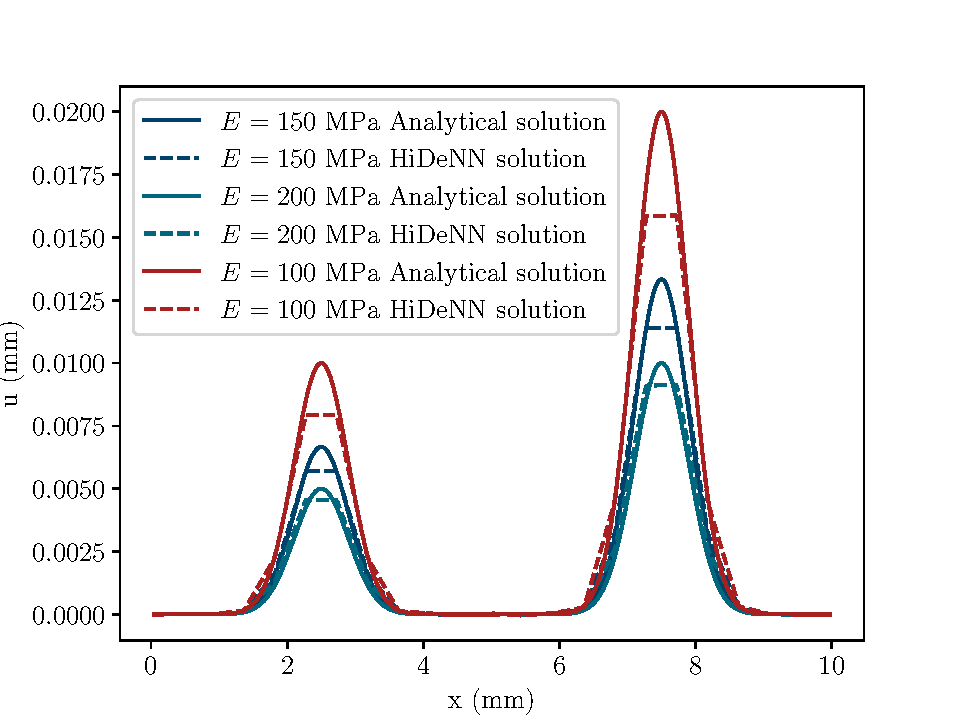
\includegraphics[width=\linewidth]{Figures/Para_displacements_np_23.pdf}
    \caption{$n_p=23$}
\end{subfigure}
  \begin{subfigure}[t]{0.5\linewidth}
    \centering
    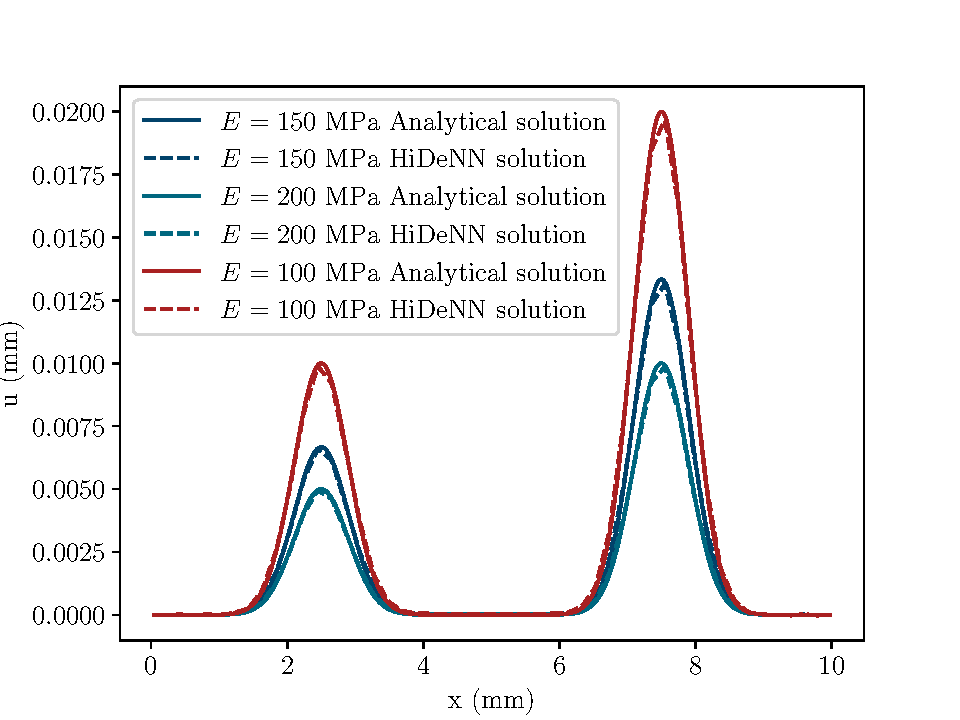
\includegraphics[width=\linewidth]{Figures/Para_displacements_np_50.pdf}
    \caption{$n_p=50$}
\end{subfigure}  
    \caption{Parametric displacement field }
    \label{fig:Para_disp}
\end{figure}



The analytical solution being
\begin{equation}
    \begin{split}
        \vect{u} = \frac{1}{AE} \left(\exp\left(- \pi \left( x-x_1 \right)^2 \right) - \exp\left(- \pi x_1^2\right) \right) &+ \frac{2}{AE} \left(\exp\left(- \pi \left( x-x_2 \right)^2 \right)  - \exp\left(- \pi x_2^2\right) \right) \\ 
        &- \frac{\exp\left(- \pi x_1^2\right) -\exp\left(- \pi x_2^2\right) }{10AE}x, 
    \end{split}
\end{equation}
it can indeed be written using exactly one mode as
\begin{equation}
     \vect{u}\left(\vect{x},E\right) = \vect{\overline{u}}\left(\vect{x}\right)\lambda\left(E\right),
\end{equation}
with
\begin{equation}
    \begin{cases}
       \begin{split}\vect{\overline{u}} = \frac{1}{A} \left(\exp\left(- \pi \left( x-x_1 \right)^2 \right) - \exp\left(- \pi x_1^2\right) \right) &+ \frac{2}{A} \left(\exp\left(- \pi \left( x-x_2 \right)^2 \right)  - \exp\left(- \pi x_2^2\right) \right) \\ 
        &- \frac{\exp\left(- \pi x_1^2\right) -\exp\left(- \pi x_2^2\right) }{10A}x, 
    \end{split}\\
        \lambda(E) = \frac{1}{E}
    \end{cases}
\end{equation}

\Rqs{In this simple example only 1 mode is required. When multiple modes are requested they all get the same weight (not looked for in a greedy manner) and therefore are all as important as one another as illustrated in \cref{fig:FullFieldsModeWeight}. The weighting always seems to be carried by the space mode as shown in \cref{fig:SpaceModeWeight,fig:ParaModeWeight} where only the magnitude of the space modes varies with the number of modes and the magnitudes of the parameter modes stay the same as if it was normalised. }{This behaviour must be linked to the different stage of training. At first only the space modes moves then when it is somewhat correct, the parameters start moving}

\Rqs{This behaviour is expected for an \emph{a priori} method where several modes are computed at once, the contributions are somewhat merged together}{This is due to the fact that no constraint on getting a orthogonal basis is made. 
\begin{itemize}
    \item Add the constraint in the loss ?
    \item Use a classical Gramm-Schmidt algorithm as a post-process 
\end{itemize}}

\Rq{When initialising with 1 mode and the other set to 0, the modes start to differentiate (the latter stay at 0 if not required). See \cref{fig:InitialisationModes}}

\begin{figure}
    \begin{subfigure}{0.3\linewidth}
        \centering
        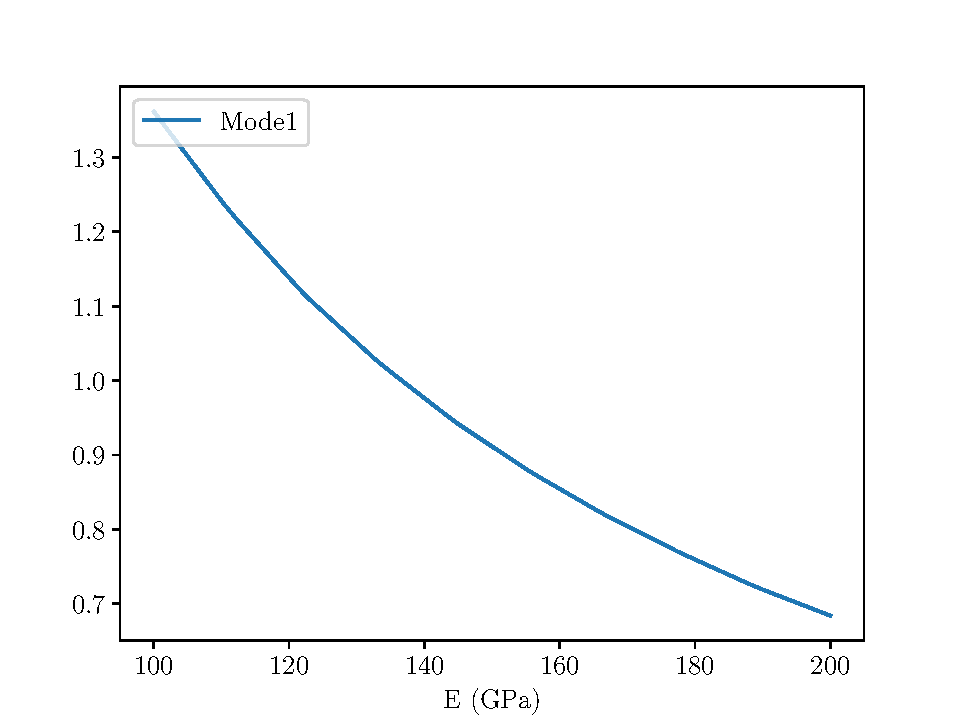
\includegraphics[width=\linewidth]{Figures/Para_modes1.pdf}
        \caption{Parametric modes for a \\$1$ mode decomposition}
    \end{subfigure}
    \begin{subfigure}{0.3\linewidth}
        \centering
        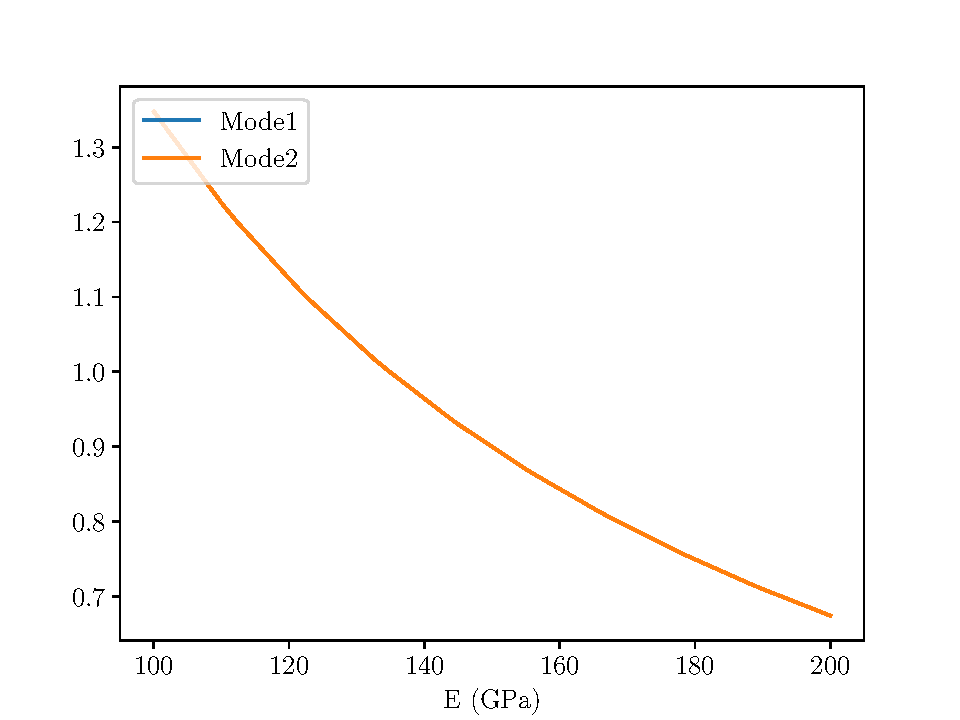
\includegraphics[width=\linewidth]{Figures/Para_modes2.pdf}
        \caption{Parametric modes for a \\$2$ modes decomposition}
    \end{subfigure}
    \begin{subfigure}{0.3\linewidth}
        \centering
        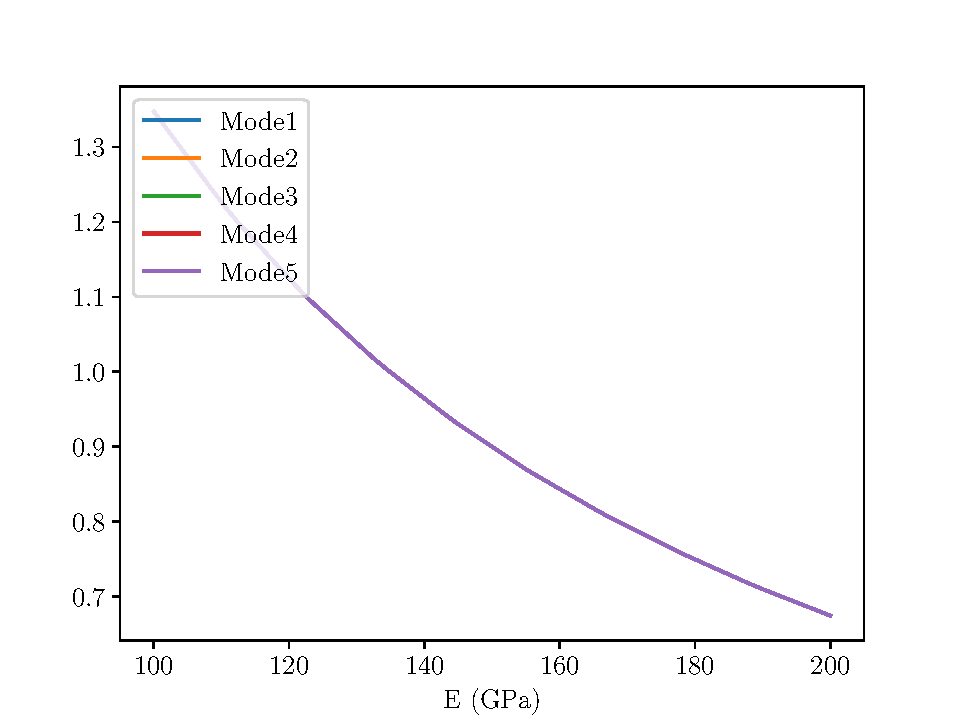
\includegraphics[width=\linewidth]{Figures/Para_modes5.pdf}
        \caption{Parametric modes for a \\$5$ modes decomposition}
    \end{subfigure}
        \caption{Parametric modes}
    \label{fig:ParaModeWeight}
\end{figure}

\begin{figure}
    \begin{subfigure}{0.3\linewidth}
        \centering
        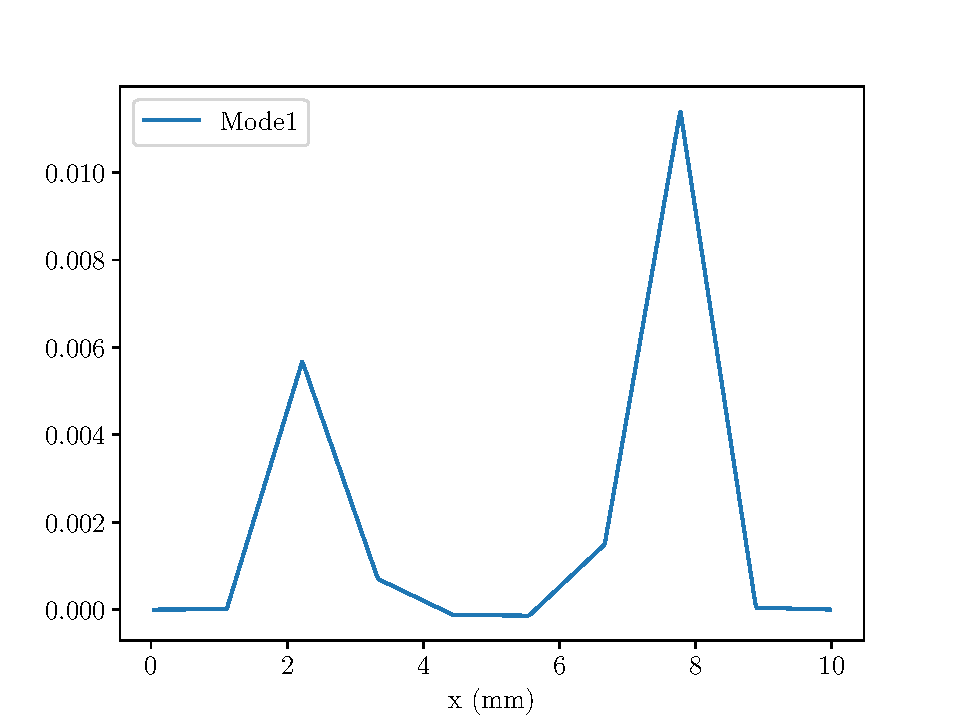
\includegraphics[width=\linewidth]{Figures/Space_modes1.pdf}
        \caption{Space modes for a \\$1$ mode decomposition}
    \end{subfigure}
    \begin{subfigure}{0.3\linewidth}
        \centering
        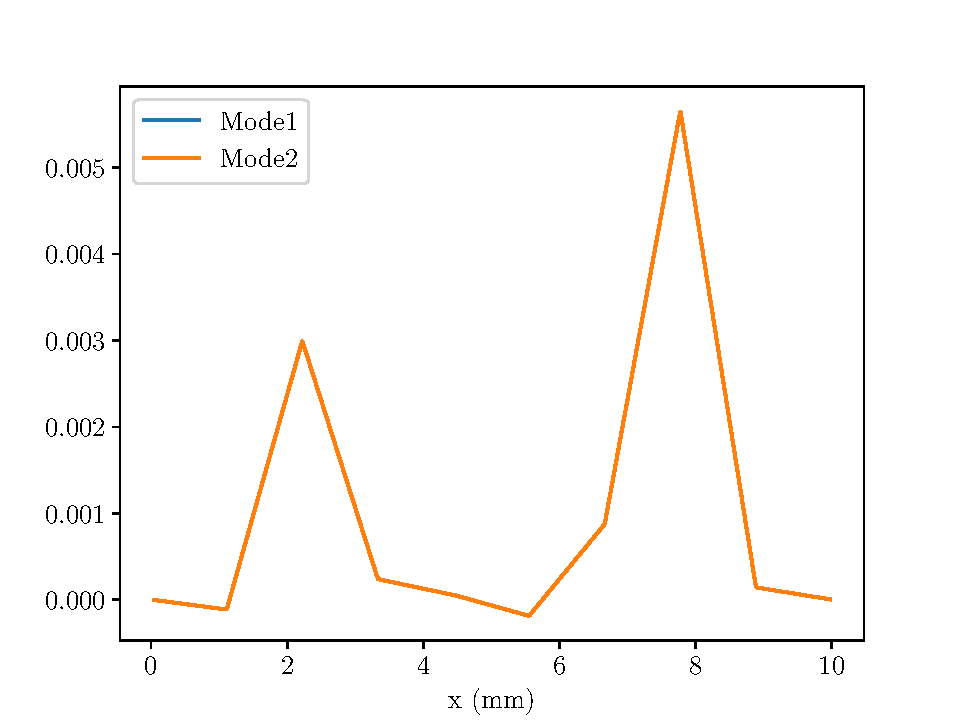
\includegraphics[width=\linewidth]{Figures/Space_modes2.pdf}
        \caption{Space modes for a \\$2$ modes decomposition}
    \end{subfigure}
    \begin{subfigure}{0.3\linewidth}
        \centering
        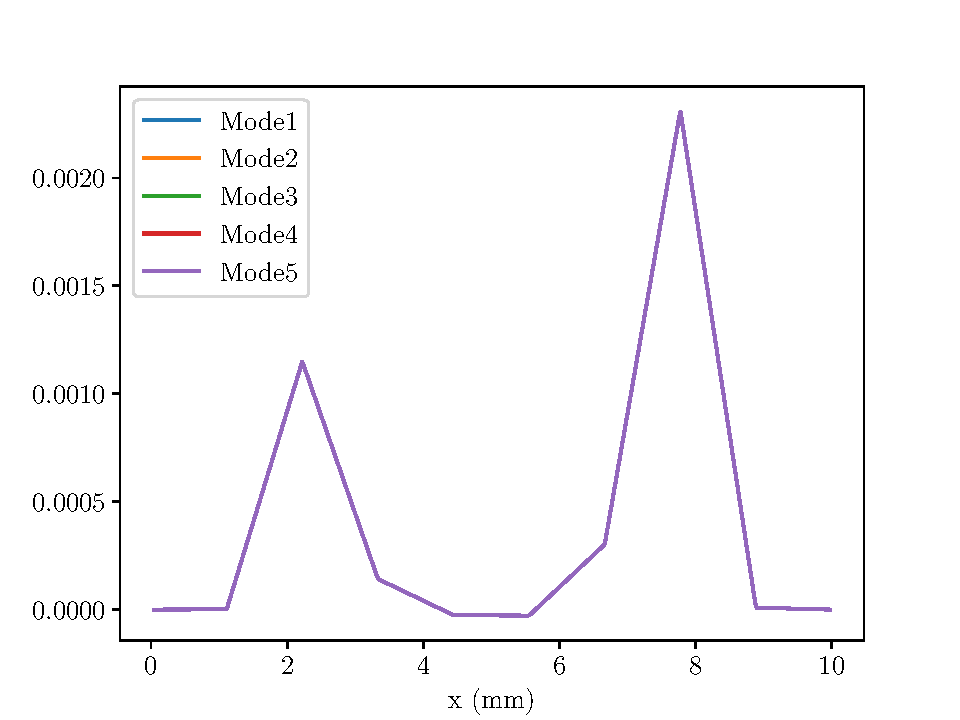
\includegraphics[width=\linewidth]{Figures/Space_modes5.pdf}
        \caption{Space modes for a \\$5$ modes decomposition}
    \end{subfigure}
        \caption{Space modes}
    \label{fig:SpaceModeWeight}
\end{figure}

\begin{figure}
    \begin{subfigure}{0.3\linewidth}
        \centering
        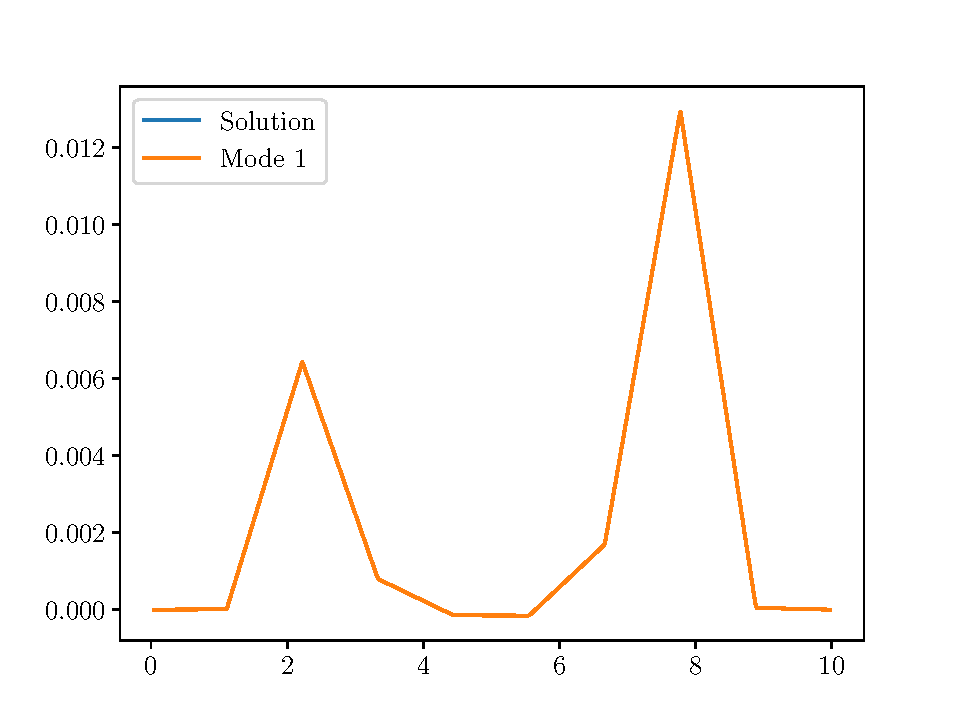
\includegraphics[width=\linewidth]{Figures/Comp_full_fields1.pdf}
        \caption{Modes contributions for a \\$1$ mode decomposition}
    \end{subfigure}
    \begin{subfigure}{0.3\linewidth}
        \centering
        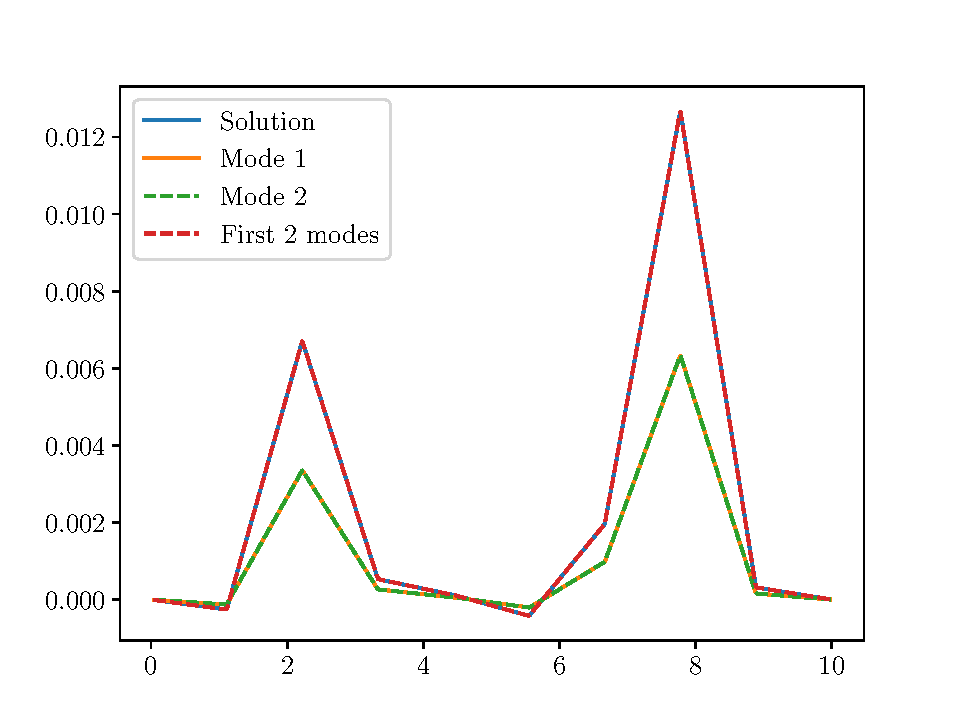
\includegraphics[width=\linewidth]{Figures/Comp_full_fields2.pdf}
        \caption{Modes contributions for a \\$2$ modes decomposition}
    \end{subfigure}
    \begin{subfigure}{0.3\linewidth}
        \centering
        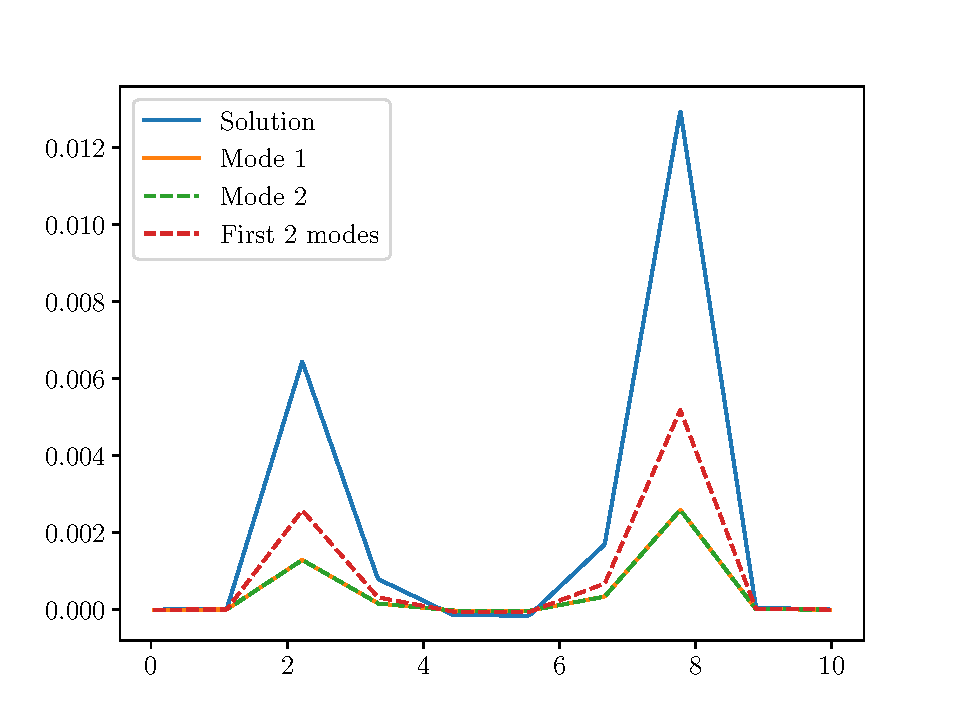
\includegraphics[width=\linewidth]{Figures/Comp_full_fields5.pdf}
        \caption{Modes contributions for a \\$5$ modes decomposition}
    \end{subfigure}
        \caption{Modes contributions}
    \label{fig:FullFieldsModeWeight}
\end{figure}

\begin{figure}
    \begin{subfigure}[t]{0.5\linewidth}
        \centering
        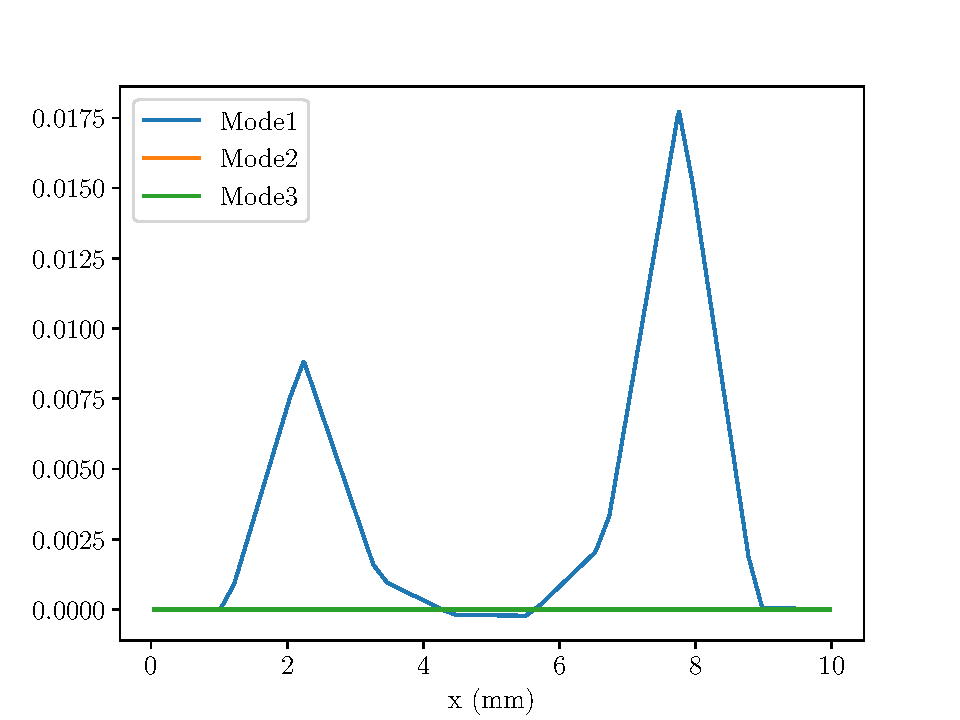
\includegraphics[width=\linewidth]{Figures/Pre_trained_Space_modes3.pdf}
        \caption{Pre-trained space mode initialisation on $1$ mode \& $n_p=10$}
    \end{subfigure}
    \begin{subfigure}[t]{0.5\linewidth}
        \centering
        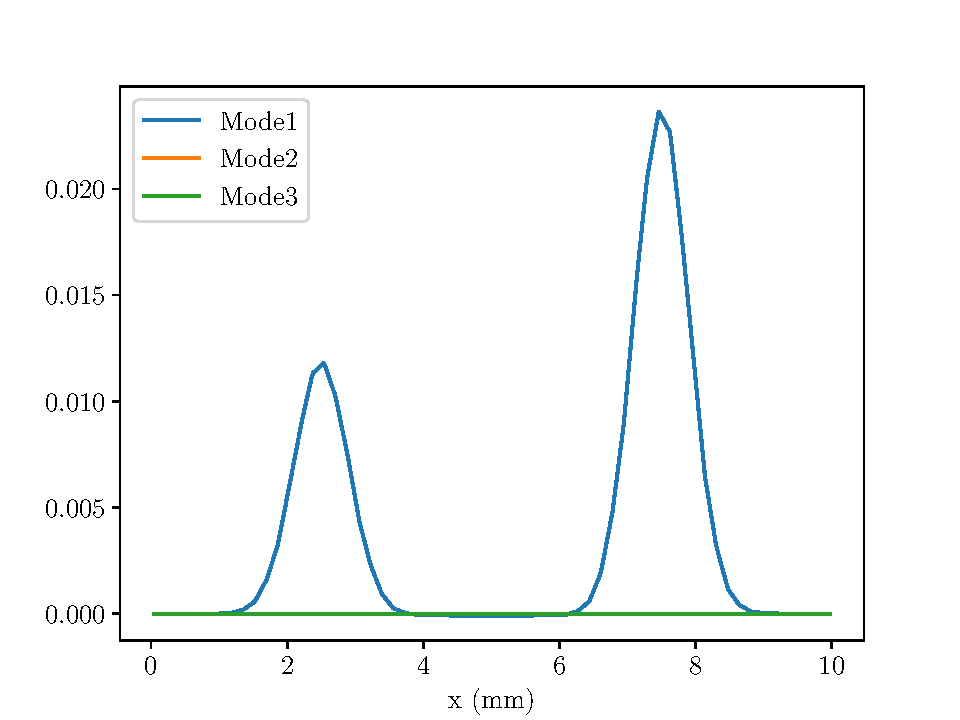
\includegraphics[width=\linewidth]{Figures/Trained_Space_modes3.pdf}
        \caption{Trained space modes}
    \end{subfigure}
    \caption{Modes initialisation (from 1 mode \& $n_p=10$ to $3$ modes \& $n_p=50$.}
    \label{fig:InitialisationModes}
\end{figure}




\subsection{Multiple parameters}

Similarly, multiple parameters can be used as extra coordinates in the tensor decomposition, leading to the expression 
    \begin{equation}
        \vect{u}\left(\textcolor{BleuLMS!70}{\vect{x}}, \textcolor{LGreenLMS}{\left\{\mu_i\right\}_{i \in \llbracket 1, \beta \rrbracket}}\right) = \sum\limits_{i=1}^m \textcolor{BleuLMS!70}{\overline{\vect{u}}_i(\vect{x})} ~\textcolor{LGreenLMS}{\prod_{j=1}^{\beta}\lambda_i^j(\mu^j)}.
    \end{equation}

The architecture presented in Figure~\ref{fig:HiDeNN_TD_mu} can be extended by adding several interpolation blocks to account for the several parameters in the tensor decomposition. Figure~\ref{fig:HiDeNN_TD_multipleMu} gives an example of such a decomposition.

\subsubsection{Spatial parameter field}
\label{sec:SpatialParameters}
In the medical context of interest, not all parameters are scalars; some are spatial fields. For such parameters, a specific representation is required for those to fit in the HiDeNN framework, which is mesh-less in that the input is coordinate-based and does not rely on a given discretisation. 

The idea is to project a given spatial field $\mu\left(x\right)$ onto a suitable basis $\left\{f_k\right\}_{k \in \llbracket 1, \beta \rrbracket}$ such that 
\begin{equation}
    \mu\left(x\right) = \sum\limits_{k=1}^{\beta}\mu^{k}f^k\left(x\right).
\end{equation}

This projection gives a set of ``patient specific'' parameters $\textcolor{LGreenLMS}{\left\{\mu^k\right\}_{k \in \llbracket 1, \beta \rrbracket}}$ that can be fed in the NN. The field $\mu\left(x\right)$ is reconstructed to compute the loss 
\begin{equation}
\mathcal{L} = g\left(\vect{u}\left((\textcolor{BleuLMS!70}{\vect{x}},\textcolor{LGreenLMS}{\left\{\mu^k\right\}}\right),\textcolor{BleuLMS!70}{\vect{x}},\mu\left(x\right)\right)
\end{equation}
as a function $g$ of quantities of interest.
\subsubsection{Illustration}
\label{1D_NeuROM_Bi}
The case of a 2-stiffness beam is illustrated.

% \begin{equation}
%     E(x) = \begin{cases}
%         E1, \forall x \in \[0,L/2\] \\
%         E2, \forall x \in \[L/2,L\]
%     \end{cases}
% \end{equation}

$$
E(x) =
\begin{cases}
E1,\quad \forall x \in \left[0,L/2\right],\\
E2,\quad \forall x \in \left[L/2,L\right]

\end{cases}
$$

\begin{figure}
    \begin{subfigure}[t]{0.5\linewidth}
        \centering
        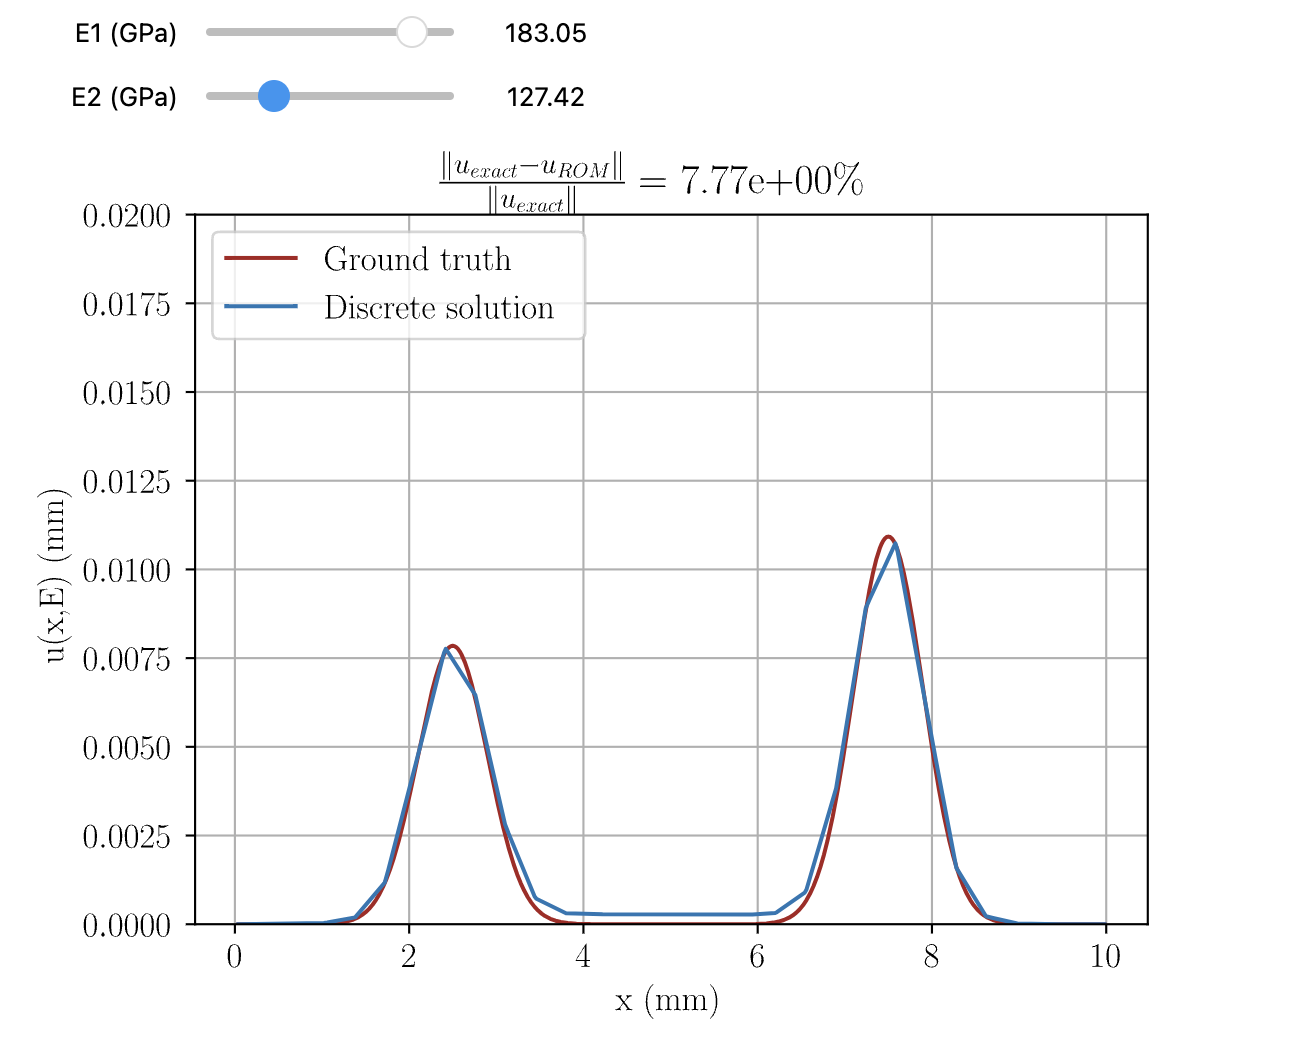
\includegraphics[width=\linewidth]{Figures/BiPara1.png}
        \caption{Config 1}
    \end{subfigure}
    \begin{subfigure}[t]{0.5\linewidth}
        \centering
        \includegraphics[width=\linewidth]{Figures/BiPara2.png}
        \caption{Config 2}
    \end{subfigure}
    \caption{Bi-parametric NeuROM}
    \label{fig:BiParam}
\end{figure}

\subsection{Operations}

\Rqs{All operations on the assemble field $\vect{u}\left(\vect{x},\vect{\mu} \right)$ are performed on the TD directly so that the cost is much lower. For instance the spatial derivative of the displacement field is computed as 
\begin{equation}
    \frac{\mathrm{d}}{\mathrm{d}x}\vect{u}\left(\vect{x},\vect{\mu} \right) = \sum\limits_{i=1}^m \textcolor{BleuLMS!70}{\frac{\mathrm{d}\overline{\vect{u}}_i(\vect{x}) }{\mathrm{d}x}} ~\textcolor{LGreenLMS}{\prod_{j=1}^{\beta}\lambda_i^j(\mu^j)}.
\end{equation}}{In the non-linear interpolation framework, need to compute the derivative of the non-linear function of $NN\left(\vect{\overline{u}}\left(\vect{x}\right)\right)$}




\subsection{Miscellaneous}
\Rqs{Each PGD modes are computed on an independent mesh, hence the localised correction of latter modes can lead to specific mesh refinement.\newline
\noindent
\textcolor{LGreenLMS}{\faLightbulb} This could solve the issue mentioned in \cref{chap:MethodPapers} in \cref{ParaRefinement}.}{A choice of allowing extrapolation or not w.r.t the parameters is possible. By default extrapolation allowed but user need to be careful.}

Regarding the reduced-order basis orthogonality:
\begin{itemize}
    \item Add the constraint in the loss ?
    \item Use a classical Gramm-Schmidt algorithm as a post-process 
\end{itemize}

\begin{itemize}
    \item Using the orthogonality of the basis and look at the downgrading coefficient to asses the quality of the basis ? If the remaining vector after the Grtam-Schmidt but before the normalisation is small it means that the basis is already sufficient, else it means that is needs to be extended. 
\end{itemize}
\subsection{Perspectives \& open questions}

This framework has only been used in the context of spatial coordinates (space-separated TD) for linear equations (with a maximum of 3 parameters). 

\begin{itemize}
    \item Large number of parameters
    \item Extra-coordinates (parameters other than spatial coordinates)
    \item Spatial parameter fields
    \item Time PDE's 
    \item PGD, \emph{i.e}, adapt on the fly the number of modes
    % \item Compare to PGD on simple equations?
    % \begin{itemize}
    %     \item Modes are computed without fixed-point algo
    %     \item Better behaviour in high dimensions is expected
    % \end{itemize}
    \item Add a layer of pre-processing of the $\mu$'s?
    \begin{itemize}
        \item Scaling, etc.
    \end{itemize}
    \item[\textcolor{RougeLMS}{\faLock}] This implementation does not allow for the mesh to be a function of the parameters
    \item[\textcolor{LGreenLMS}{\faCheckCircle }] Allow to have \emph{in between trainable layers} that do function compositions of the modes to get nonlinear interpolations
        \begin{itemize}
        \item Take up the general idea put forward by \cite{kramer_learning_2024,geelen_learning_2023} but extend it to automate the nonlinear combination  without prior knowledge of the required interpolation as opposed to guessing polynomial combinations.
        \item The low rank field would read $\vect{u}\left(\textcolor{BleuLMS!70}{\vect{x}}, \textcolor{LGreenLMS}{\left\{\mu_i\right\}_{i \in \llbracket 1, \beta \rrbracket}}\right) = \sum\limits_{i=1}^m \textcolor{BleuLMS!70}{f\left(\overline{\vect{u}}_i(\vect{x})\right)} ~\textcolor{LGreenLMS}{\prod_{j=1}^{\beta}g\left(\lambda_i^j(\mu^j)\right)}$, 
        with $f$ and $g$ arbitrary functions of the modes, learned by the neural network in the reduced-order space so that the learning cost is lower but we achieve better reductibility by using non-linear combinations of the modes instead of increasing drastically the number of modes required.
    \end{itemize}
    \item[\textcolor{LGreenLMS}{\faCheckCircle }] Does not rely on a prior discretisation of the parameters (Thanks to the continuous interpolation given by the shape functions)
\end{itemize}


\section{Boundary conditions}
\label{BCs_TD}




In order to account for boundary conditions in the case of non homogeneous boundary conditions it is required to use a lifting of the solution. The idea is to write the solution as a sum of admissible and homogeneous (admissible to zero) fields.
To do so, the first space mode is set with the actual boudary conditions while the following modes are set up with homogeneous boundary conditions. In order not to interefer with the space boundary conditions, the parametric modes associated with the first modes are uniformly equal to one.

The displacement thus reads


    \begin{equation}
        \vect{u}\left(\textcolor{BleuLMS!70}{\vect{x}}, \textcolor{LGreenLMS}{\left\{\mu_i\right\}_{i \in \llbracket 1, \beta \rrbracket}}\right) = \underbrace{\textcolor{BleuLMS!70}{\overline{\vect{u}}_1(\vect{x})} ~\textcolor{LGreenLMS}{\prod_{j=1}^{\beta}\lambda_1^j(\mu^j)} }_{\text{Admissible field}}+ \sum\limits_{i=2}^m \underbrace{\textcolor{BleuLMS!70}{\overline{\vect{u}}_i(\vect{x})} ~\textcolor{LGreenLMS}{\prod_{j=1}^{\beta}\lambda_i^j(\mu^j)}}_{\text{Homogeneous corrections}}.
    \end{equation}

\Rqs{\begin{itemize}
    \item $\lambda_1^j(\mu^j) = 1, \forall j \in \llbracket 1,\beta \rrbracket$
    \item $\overline{\vect{u}}_1(\vect{x}) = \vect{u}_d$ on $\partial \Omega_d$
    \item $\overline{\vect{u}}_i(\vect{x}) = \vect{0}$ on $\partial \Omega_d, \forall i  \in \llbracket 2,m \rrbracket$
    \item If the number of requested modes is strictly less than $2$ in such case, it is increased to $2$ automatically.
\end{itemize}}{The first mode is kinematically admissible while the following modes are admissible to zero.}

\textbf{\textcolor{accentcolor}{Note:}} in their paper, \cite{zhang_hidenn-td_2022} utilises body forces so that they do not have to deal with non zero Dirichlet boundary conditions.

In the simple 1D bar two modes are now required to get the boundary conditions. It works just as fine as shown in \ref{fig:BCsDispl_para} but the modes are not orthogonal.
The human brain would imagine a linear mode and he same KA0 mode that ws previously obtained but the two modes are a mixed of the two as shown in \cref{fig:SpaceModesBCs}

\begin{figure}
    \centering
    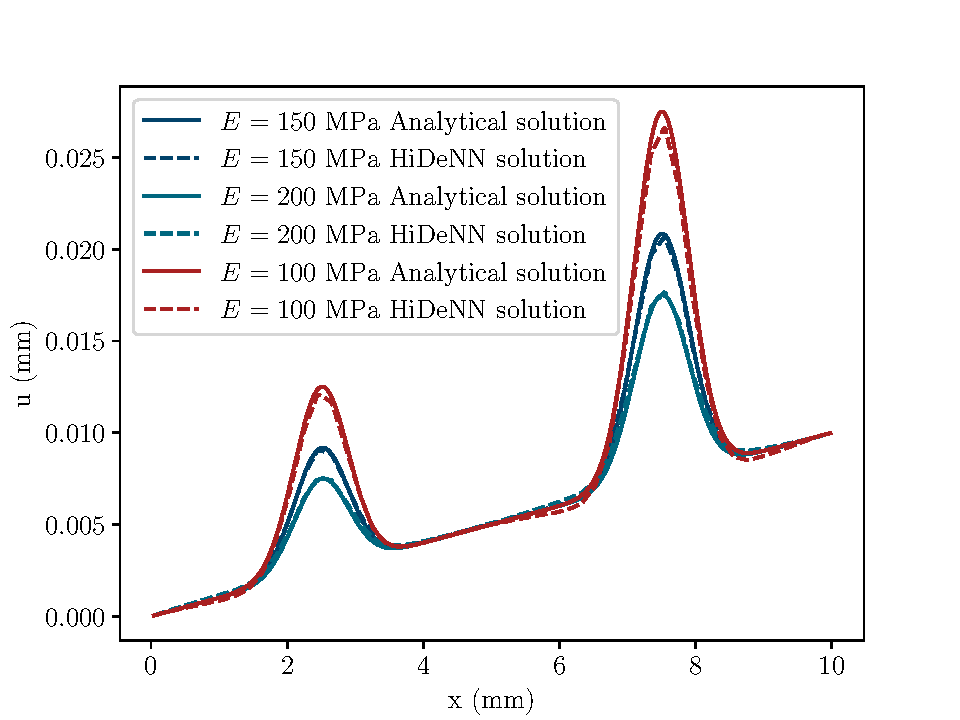
\includegraphics[width=0.7\linewidth]{Figures/Para_displacementsROM_1Para_np_50_order_1_nmodes_1_npara_1BCs.pdf}
    \caption{Parametric displacement for non homogeneous BCs}
    \label{fig:BCsDispl_para}
\end{figure}

\begin{figure}
\begin{subfigure}[t]{0.5\linewidth}
    \centering
    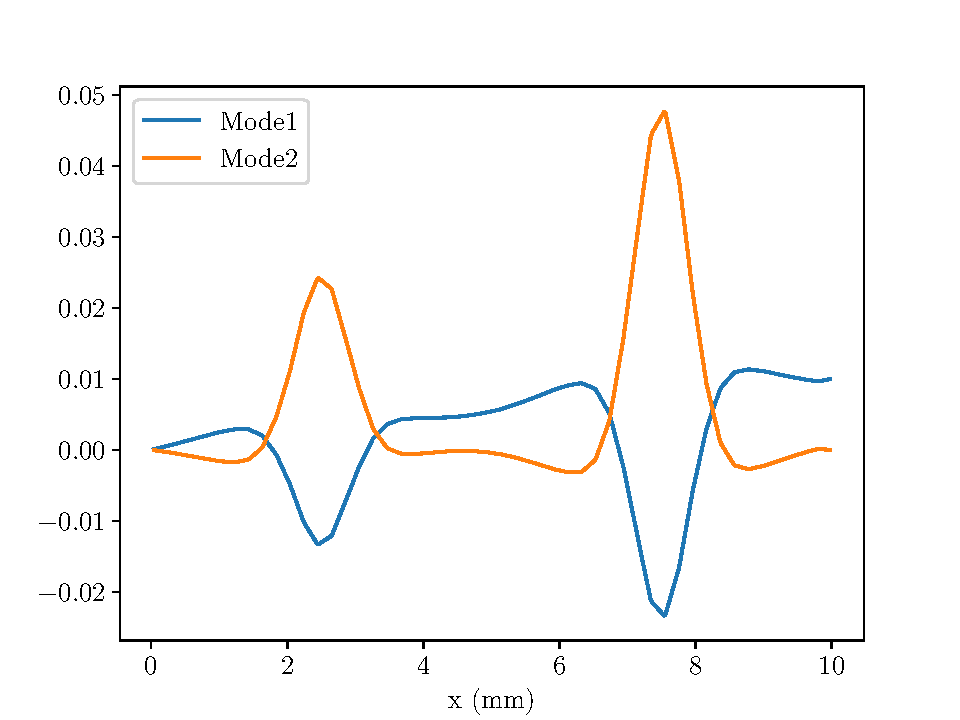
\includegraphics[width=\linewidth]{Figures/Pre_trained_Space_modes2.pdf}
    \caption{Space modes}
\end{subfigure}
  \begin{subfigure}[t]{0.5\linewidth}
    \centering
    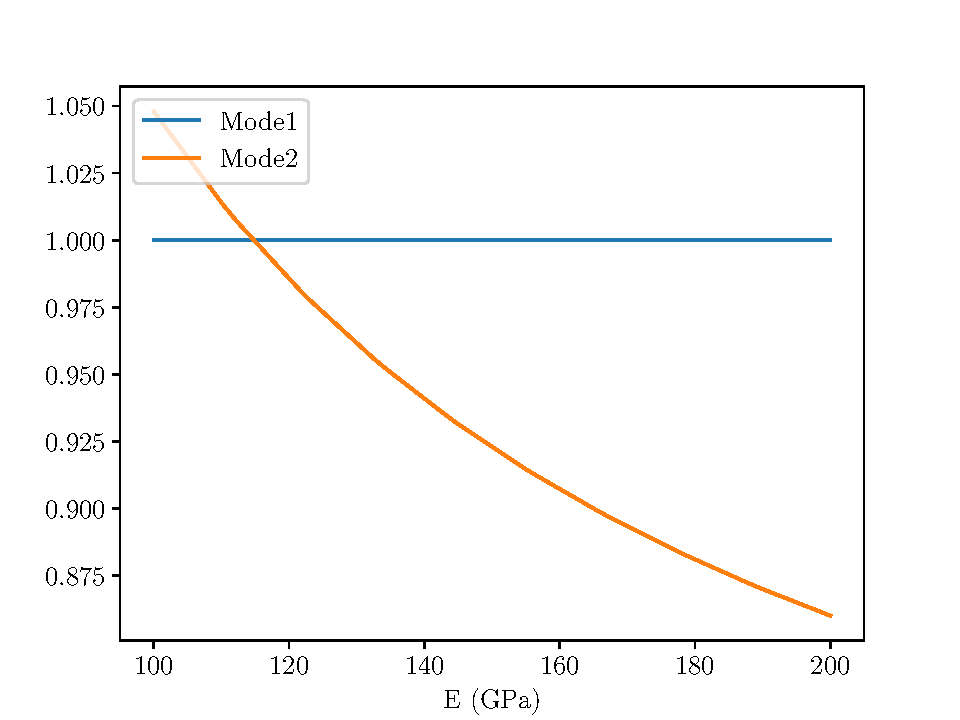
\includegraphics[width=\linewidth]{Figures/Pre_trained_Para_modes2.pdf}
    \caption{Parametric modes}
\end{subfigure}  
    \caption{Para modes}
    \label{fig:SpaceModesBCs}
\end{figure}



After an SVD the reduced-order basis is shown in \ref{fig:SVDROM_2Modes}.
\begin{figure}
\begin{subfigure}[t]{0.5\linewidth}
    \centering
    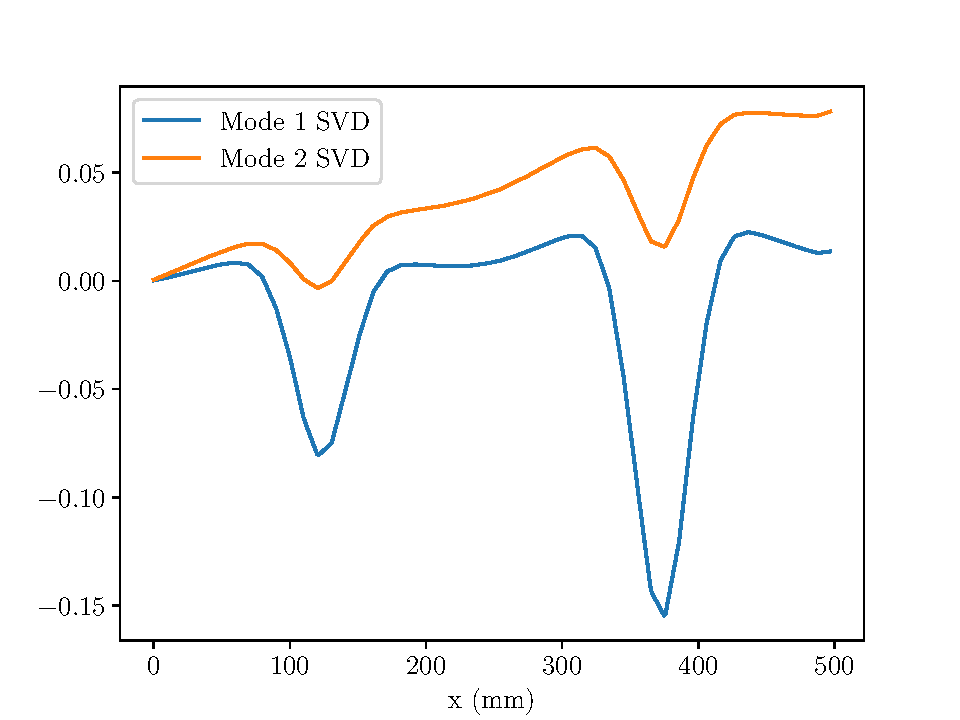
\includegraphics[width=\linewidth]{Figures/SVD_2_Modes.pdf}
    \caption{SVD of space modes }
\end{subfigure}
  \begin{subfigure}[t]{0.5\linewidth}
    \centering
    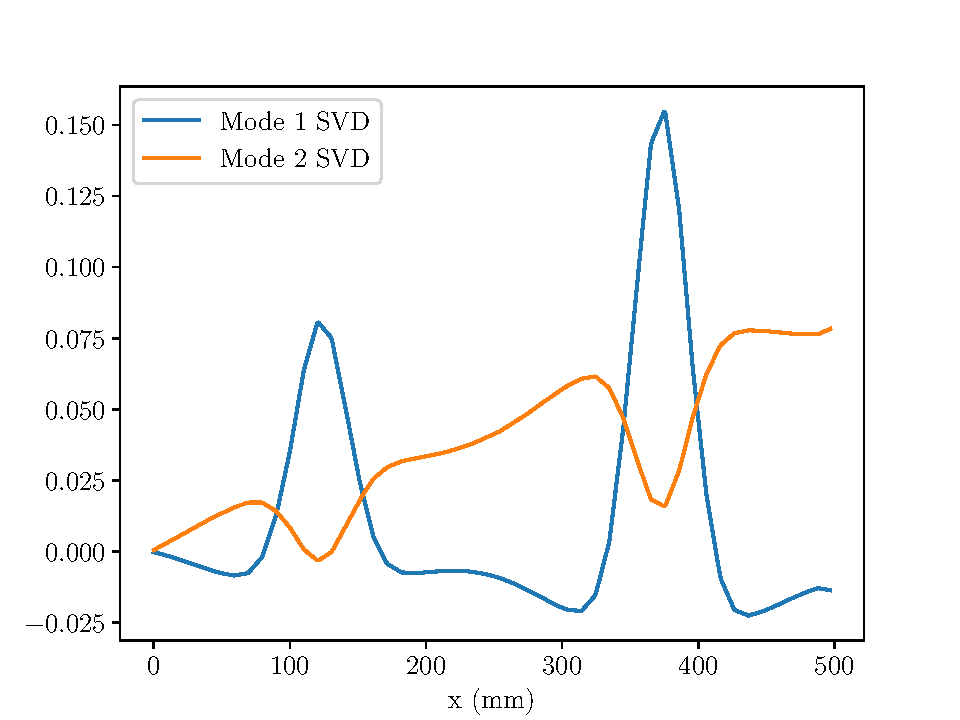
\includegraphics[width=\linewidth]{Figures/SVD_2_Modes_neg.pdf}
    \caption{SVD modes straightened ($\times -1$)}
\end{subfigure}  
    \caption{Orthogonal space modes}
    \label{fig:SVDROM_2Modes}
\end{figure}


\subsection{Initialisation} 
\paragraph{Note:} Pre trained model: $n_p = 100$, current model $n_p = 50$
Here initialising the second mode (KA0) with the first (and only) mode in case of homogeneous BCs helped a lot if frozen afterwards (see \ref{fig:BCsInitFrozen}) but lead to bad solution if free to keep evolving after initialisation (see \ref{fig:BCsInitFree}).

\begin{figure}
\begin{subfigure}[t]{0.5\linewidth}
    \centering
    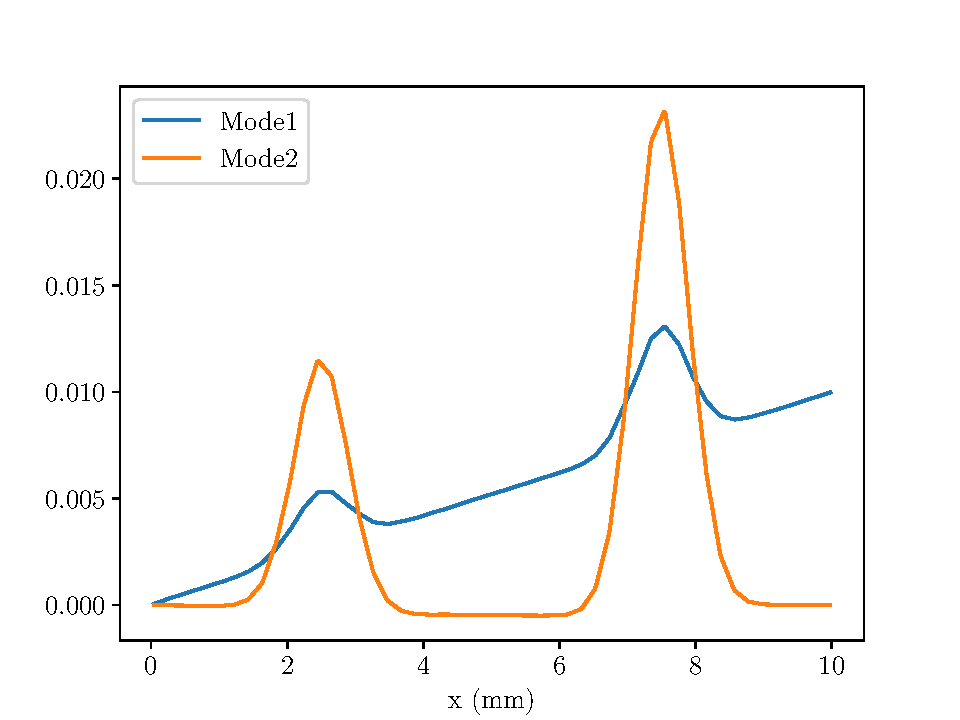
\includegraphics[width=\linewidth]{Figures/Pre_trained_Space_modes2_frozen.pdf}
    \caption{Space modes }
\end{subfigure}
  \begin{subfigure}[t]{0.5\linewidth}
    \centering
    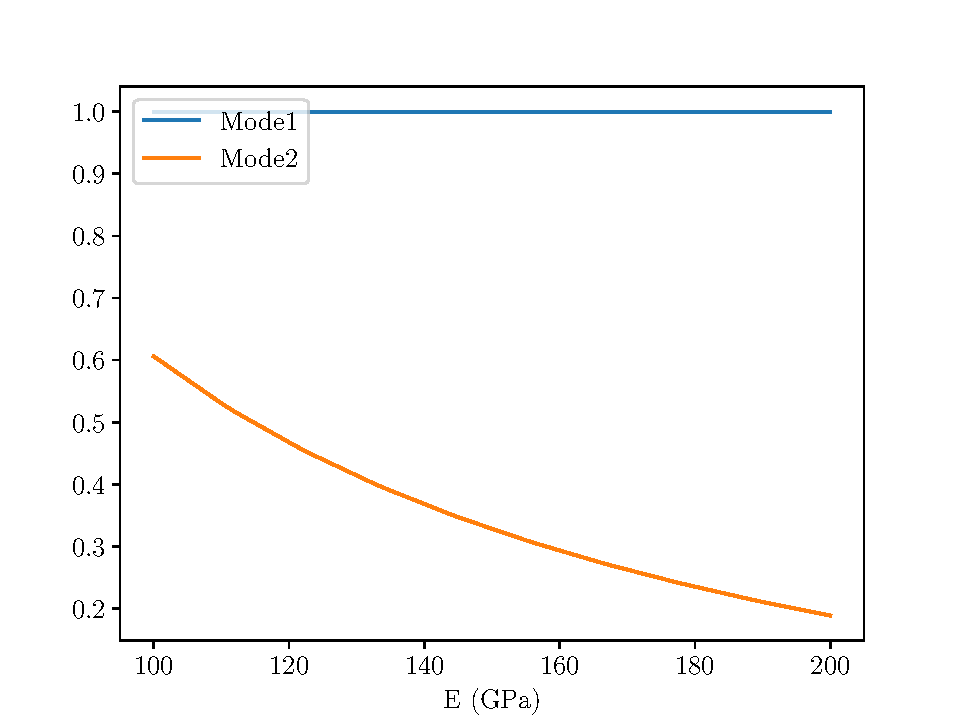
\includegraphics[width=\linewidth]{Figures/Pre_trained_Para_modes2_frozen.pdf}
    \caption{Para modes}
\end{subfigure}  
  \begin{subfigure}[t]{0.5\linewidth}
    \centering
    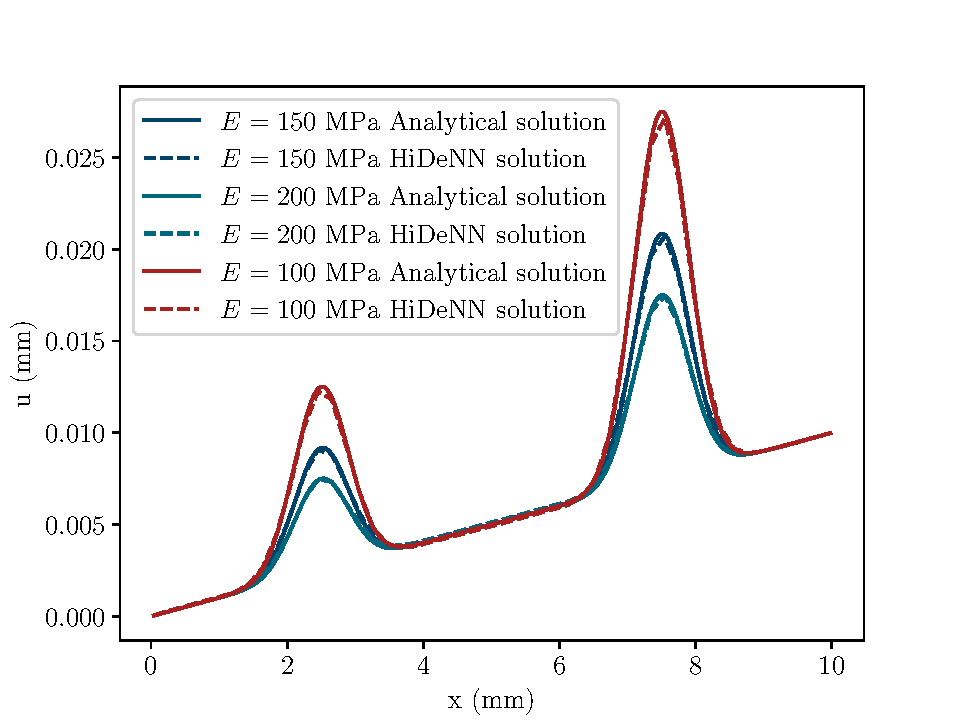
\includegraphics[width=\linewidth]{Figures/Para_displacementsROM_1Para_np_50_order_1_nmodes_1_npara_1BCs_init_frozen.pdf}
    \caption{Parametric solution}
\end{subfigure} 
  \begin{subfigure}[t]{0.5\linewidth}
    \centering
    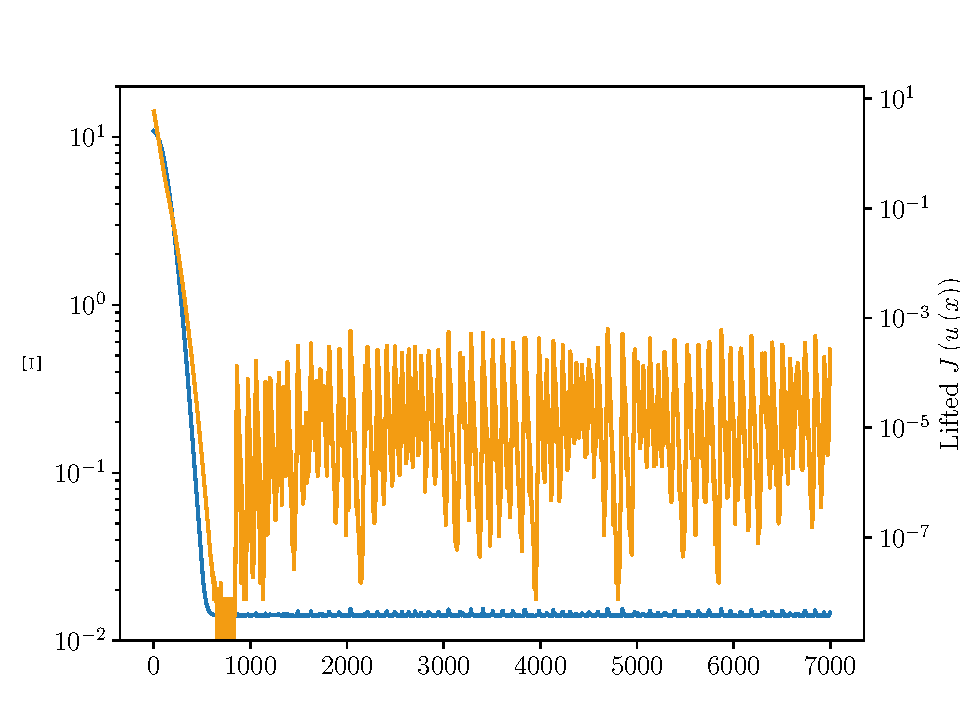
\includegraphics[width=\linewidth]{Figures/Non0BCs_init_frozen.pdf}
    \caption{Convergence of training}
\end{subfigure} 
    \caption{ROB with non zeros BCs init with $1^{\text{st}}$ mode of $0$ BCs and then frozen}
    \label{fig:BCsInitFrozen}
\end{figure}


\begin{figure}
\begin{subfigure}[t]{0.5\linewidth}
    \centering
    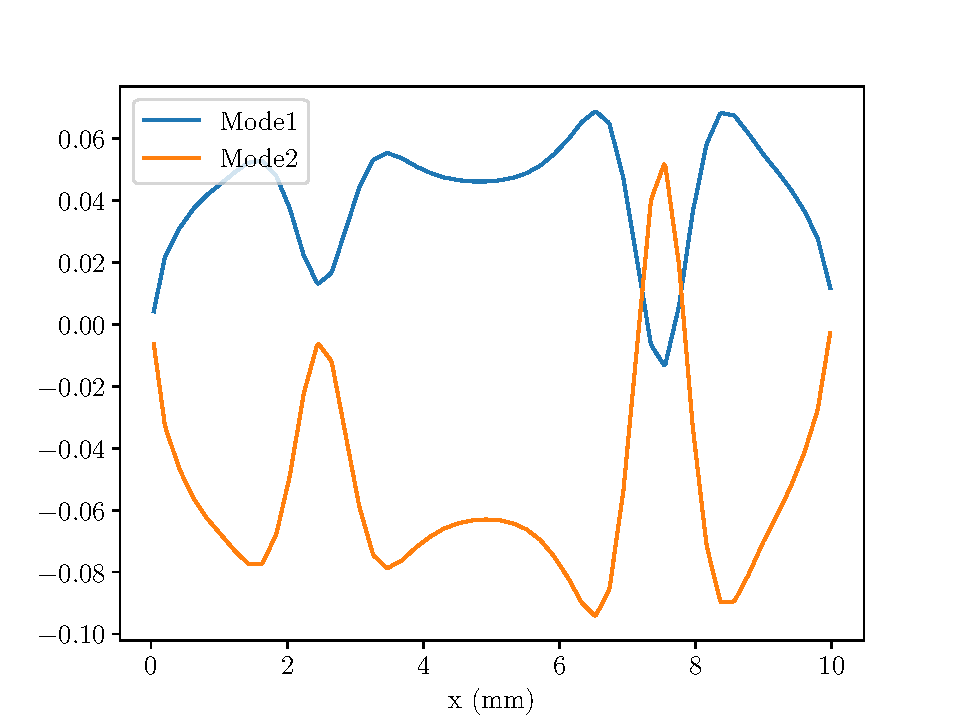
\includegraphics[width=\linewidth]{Figures/Pre_trained_Space_modes2BCs.pdf}
    \caption{Space modes}
\end{subfigure}
  \begin{subfigure}[t]{0.5\linewidth}
    \centering
    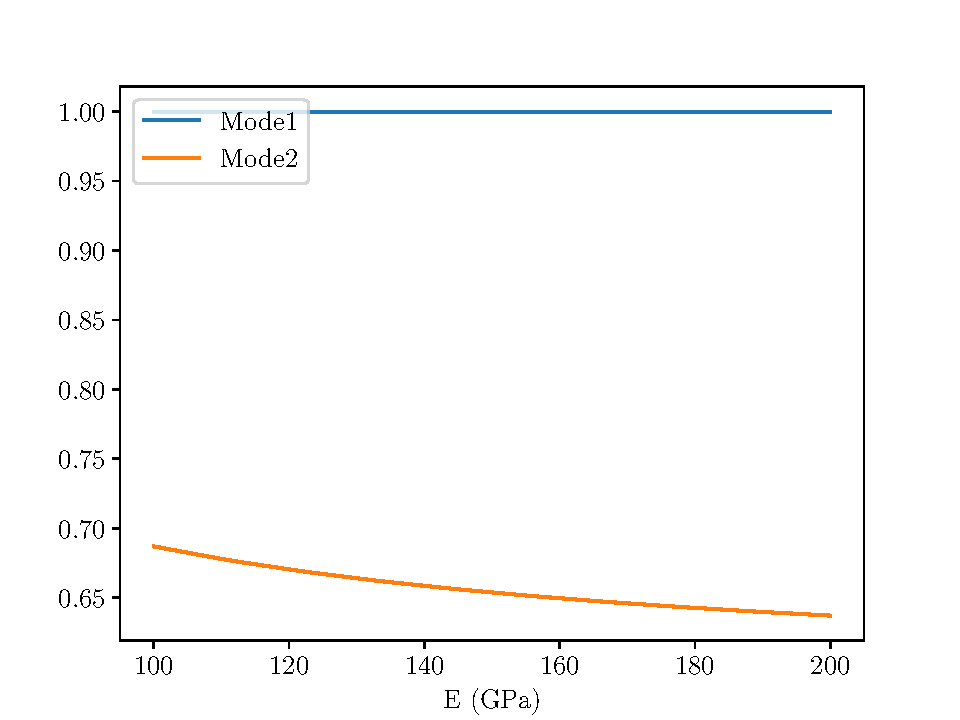
\includegraphics[width=\linewidth]{Figures/Pre_trained_Para_modes2BCs.pdf}
    \caption{Para modes}
\end{subfigure}  
  \begin{subfigure}[t]{0.5\linewidth}
    \centering
    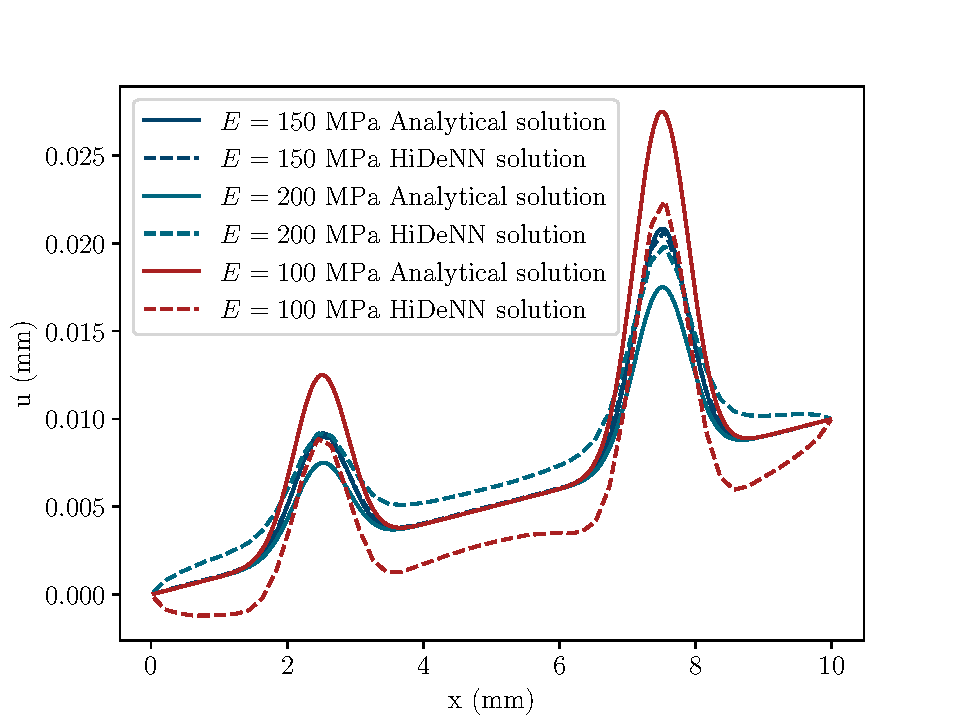
\includegraphics[width=\linewidth]{Figures/Para_displacementsROM_1Para_np_50_order_1_nmodes_1_npara_1BCs_init_free.pdf}
    \caption{Parametric solution}
\end{subfigure} 
  \begin{subfigure}[t]{0.5\linewidth}
    \centering
    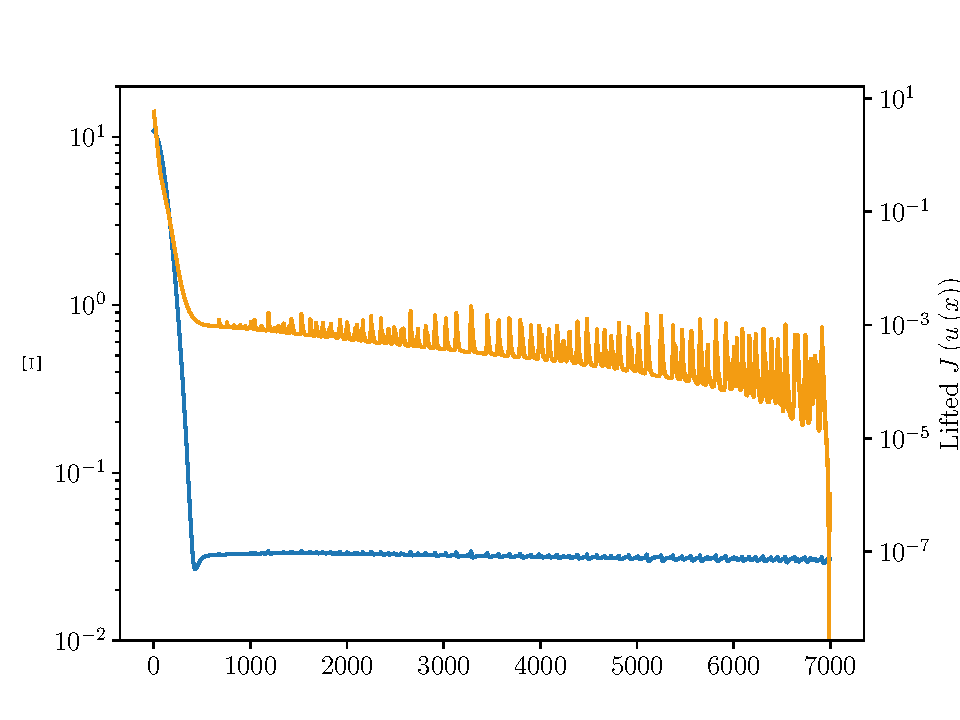
\includegraphics[width=\linewidth]{Figures/Non0BCs_init_free.pdf}
    \caption{Convergence of training}
\end{subfigure} 
\caption{ROB with non zeros BCs init with $1^{\text{st}}$ mode of $0$ BCs and then let free}
    \label{fig:BCsInitFree}
\end{figure}


If Parametric modes and space modes are frozen then we get the expected space modes and convergence is even faster as shown in \ref{fig:BCsInitFrozen_parfrozen}.

\begin{figure}
\begin{subfigure}[t]{0.5\linewidth}
    \centering
    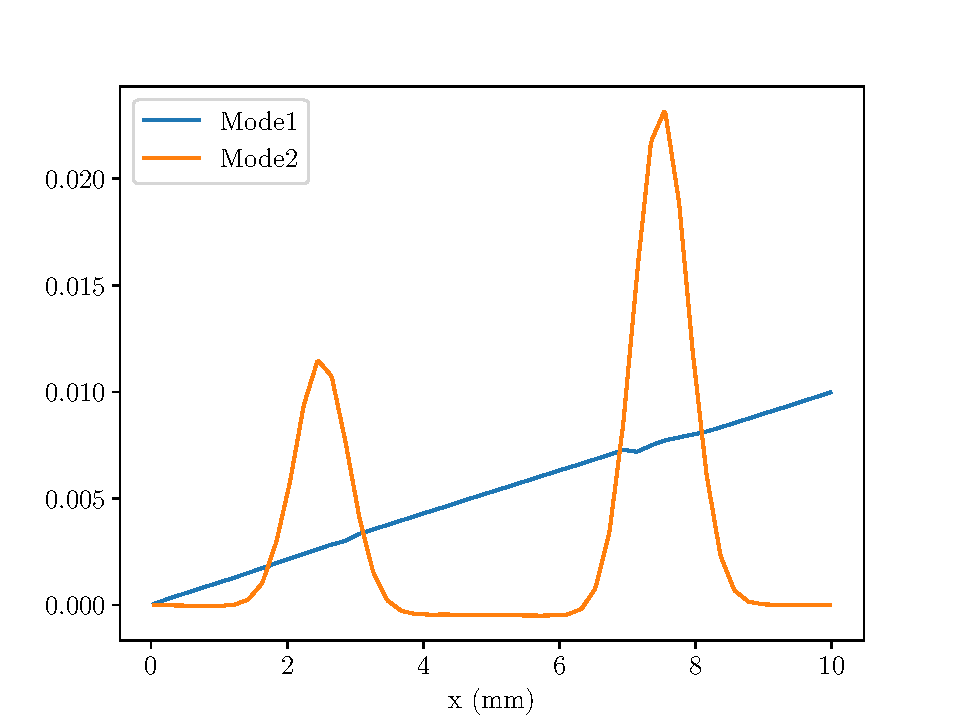
\includegraphics[width=\linewidth]{Figures/Pre_trained_Space_modes2BCs_AllFrozen.pdf}
    \caption{Space modes}
\end{subfigure}
  \begin{subfigure}[t]{0.5\linewidth}
    \centering
    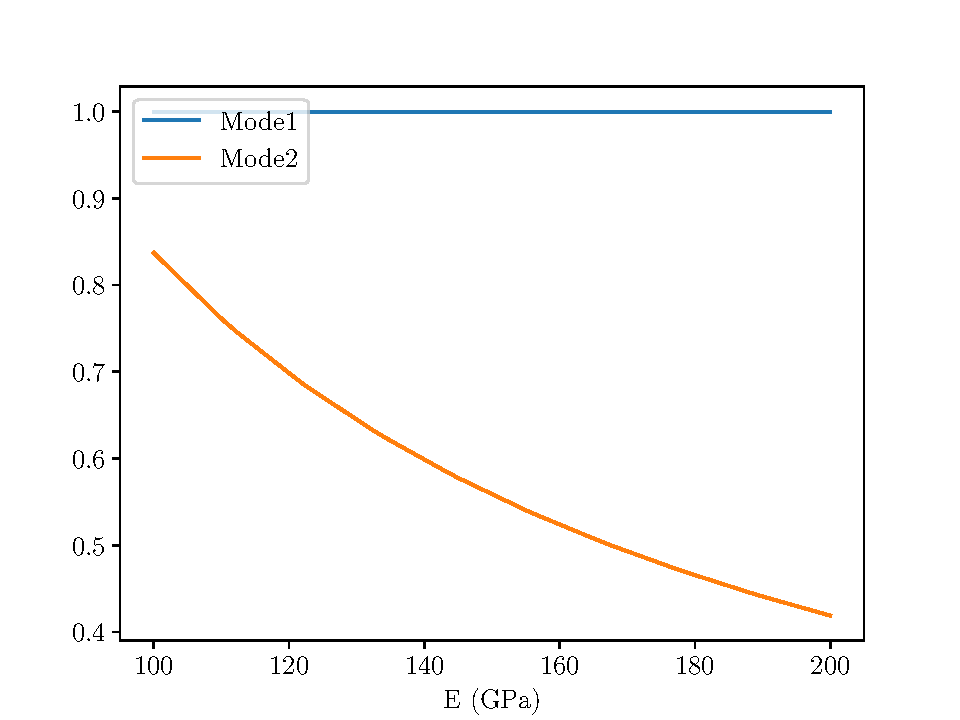
\includegraphics[width=\linewidth]{Figures/Pre_trained_Para_modes2BCs_AllFrozen.pdf}
    \caption{Para modes}
\end{subfigure}  
  \begin{subfigure}[t]{0.5\linewidth}
    \centering
    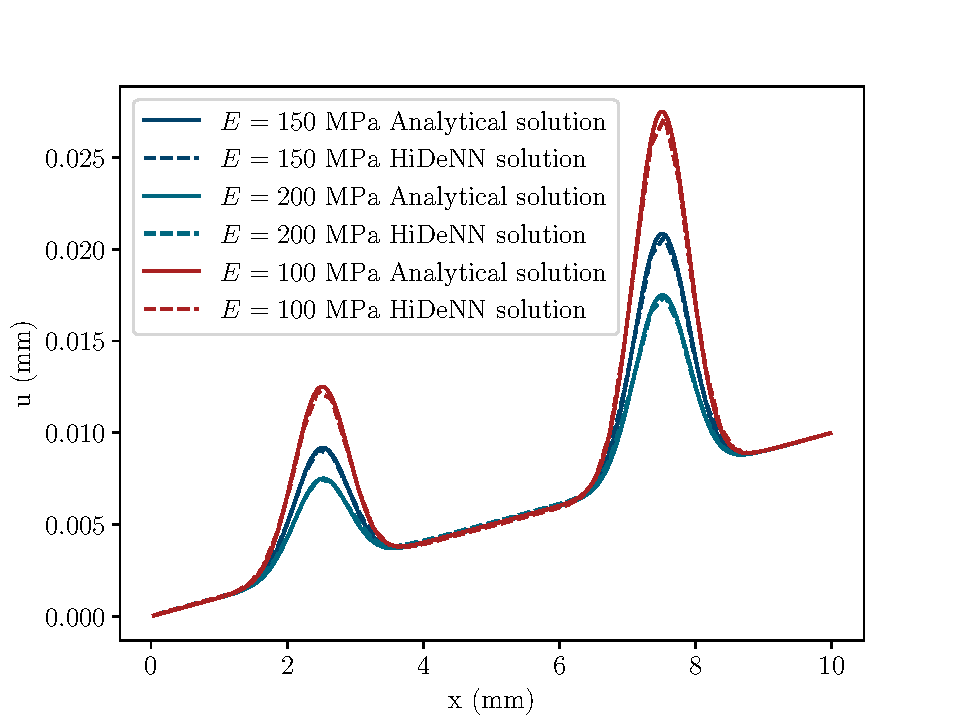
\includegraphics[width=\linewidth]{Figures/Para_displacementsROM_1Para_np_50_order_1_nmodes_1_npara_1BCs_init_all_frozen.pdf}
    \caption{Parametric solution}
\end{subfigure} 
  \begin{subfigure}[t]{0.5\linewidth}
    \centering
    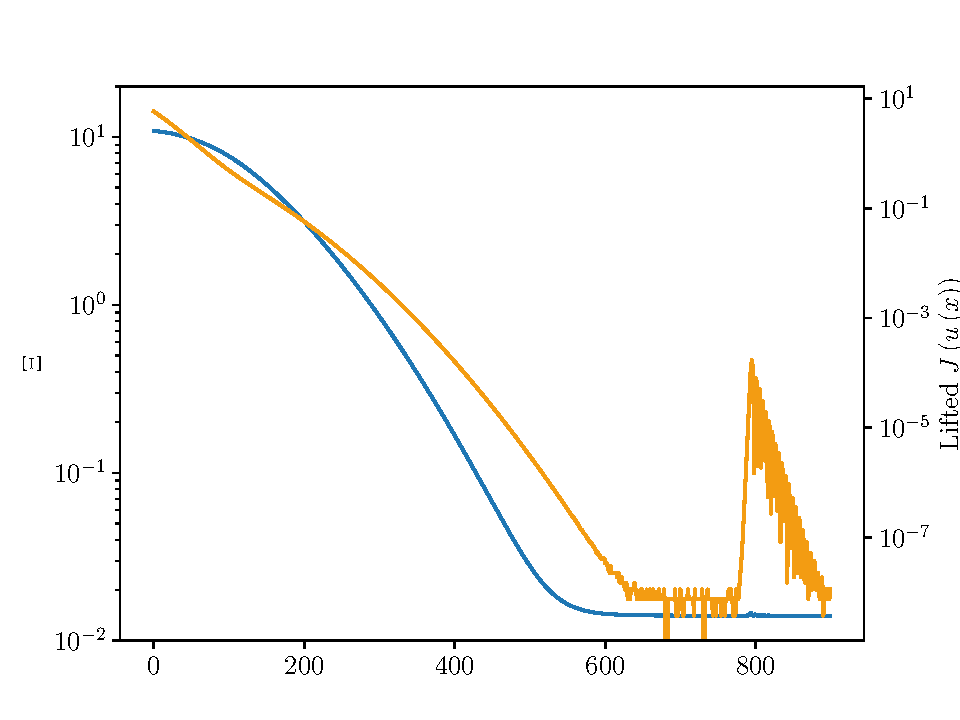
\includegraphics[width=\linewidth]{Figures/Non0BCs_init_frozen_parafrozen.pdf}
    \caption{Convergence of training}
\end{subfigure} 
\caption{ROB with non zeros BCs init with $1^{\text{st}}$ mode of $0$ BCs with both space and parametric modes frozen after initialised.}
    \label{fig:BCsInitFrozen_parfrozen}
\end{figure}

\Rq{This behaviour should be tested with Katka's new training strategy. }

\section{Identification applications}

Having a reduced-order model allows for quick and efficient model updating based on data. 

A classical gradient descent in which the frozen model is used can be implemented under the form of a neural network relying on a loss with a term relative to data fitting. Stochastic methods can also be employed rather cheaply as each query to the reduced-order model would be very inexpensive. Explicit symbolic derivative of the solution regarding the parameters would also be available.


\section{Orthogonality}
See \cref{Chap_22_03_24}, \cref{sec:orthogonality}.
\subsection{Space orthogonality constraint}
It does not allow using the TD for computing the loss but orthonormality can still be imposed at the ``Node defined'' level within the NN. The hope would be to regularise the minimisation problem and lead to a quicker training. 

In practice it seems that the reduced freedom leads, conversely, to more iterations in the gradient descent. 

\Rqs{This observation might be due to the impossibility to correct small defect in a given mode with another one due to the orthogonality constraint.}{Lifting the orthogonality constraint and imposing only a normality constraint does not help either...}

\subsection{Efficiency}

Without the orthogonality constraint, the number of operation is bound to remain higher, however it appears that the bottleneck was not due to the sole number of operation as using the Einstein's summation in a single pass, \emph{i.e.} without reconstructing the full field tensor as an intermediate step, allowed significant gains and escaping the curse of dimensionality, getting to somehow ``logical''scaling.

\section{Parametrisation of spatial fields}

For the personalising of the lung model it is important to describe the spatial field in a parameterised way in order to obtain a surrogate model whose input parameter can account for the specific stiffness field of a given patient.

The idea is to project a given spatial field $\mu\left(x\right)$ onto a suitable basis $\left\{f_k\right\}_{k \in \llbracket 1, \beta \rrbracket}$ such that 
\begin{equation}
    \mu\left(x\right) = \sum\limits_{k=1}^{\beta}\mu^{k}f^k\left(x\right).
\end{equation}

\subsection{Wavelets}

To do so while maintaining a relatively low number of parameters, we propose to project this field onto a wavelet functions basis that have proven efficient at capturing strong localised gradients.

\Rqs{On difficulty is that the $\{\mu^i\}$ from one patient to the other must be associated to the same space functions $\left\{f^i\right\}$ so that they carry the same physical meaning and the model trained for a given patient can be used for another one. }{The previous remark implies in particular that the truncation can not be preceded by a sorting of the $\left\{\mu^i\right\}$ as such an operation would be patient specific. The $N_w$ first weight will be kept no matter their decay; the truncated representation on the wavelet basis is therefore be suboptimal...}

\subsubsection{Wavelets in 1D}

A one dimensional space distribution has been parametrised with wavelet with the idea of decreasing the number of parameters required to describe it. A comparison of different space distribution and wavelet functions is shown in \cref{Wavelet_1D}.
\begin{figure}[hbpt!]
\begin{subfigure}[t]{0.5\linewidth}
    \centering
    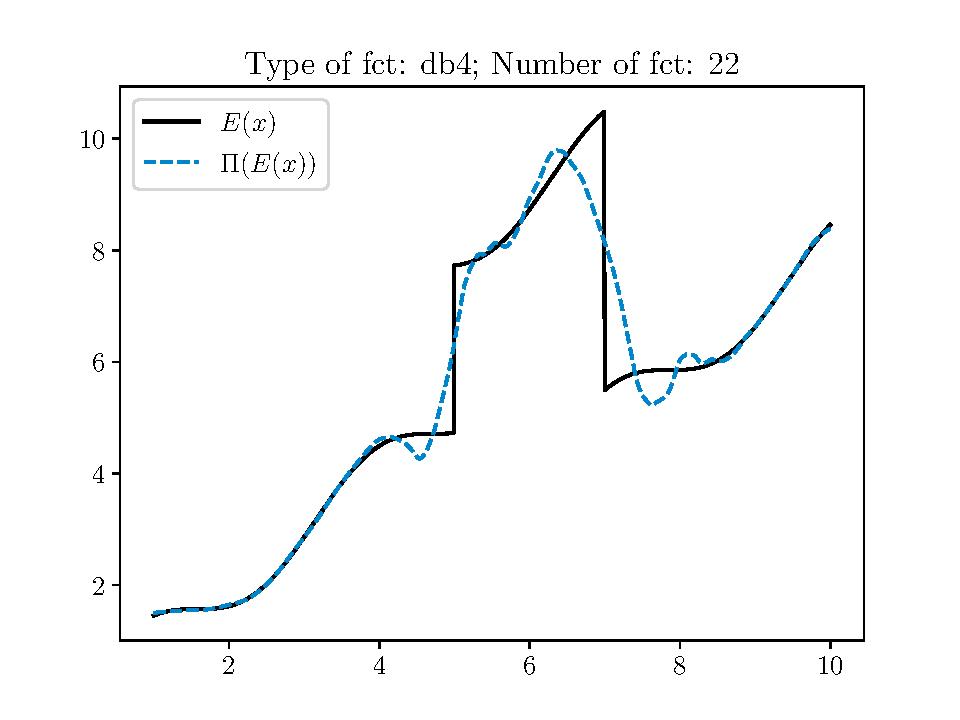
\includegraphics[width=\linewidth]{Figures/db4_N_22.pdf}
    \caption{Daubechies - smooth function}
\end{subfigure}
  \begin{subfigure}[t]{0.5\linewidth}
    \centering
    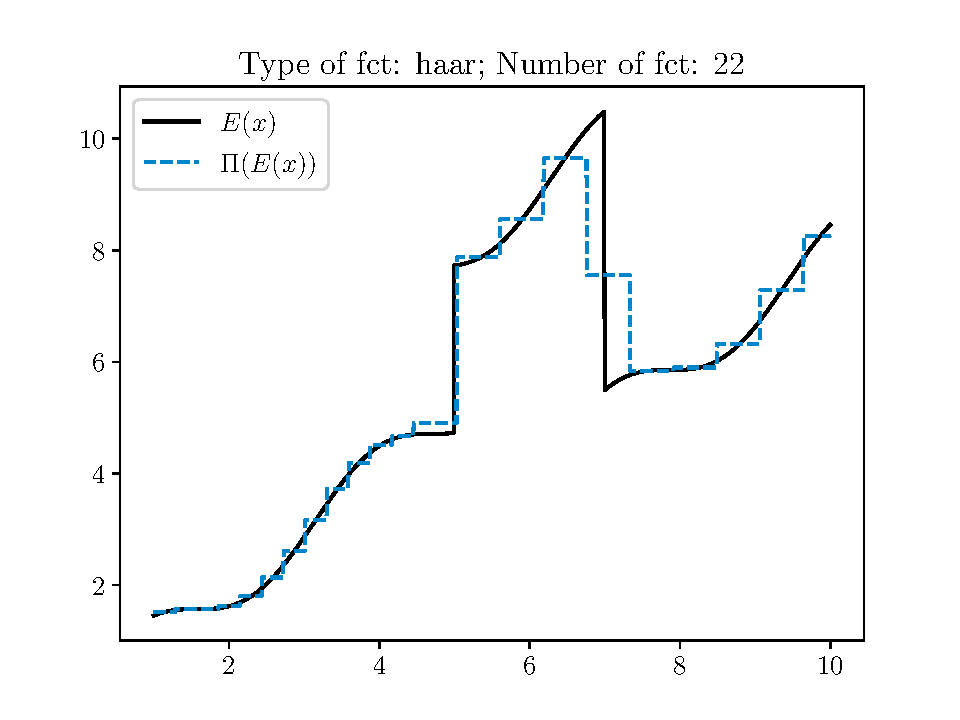
\includegraphics[width=\linewidth]{Figures/haar_N_22.pdf}
    \caption{Haar - smooth function}
\end{subfigure}  
  \begin{subfigure}[t]{0.5\linewidth}
    \centering
    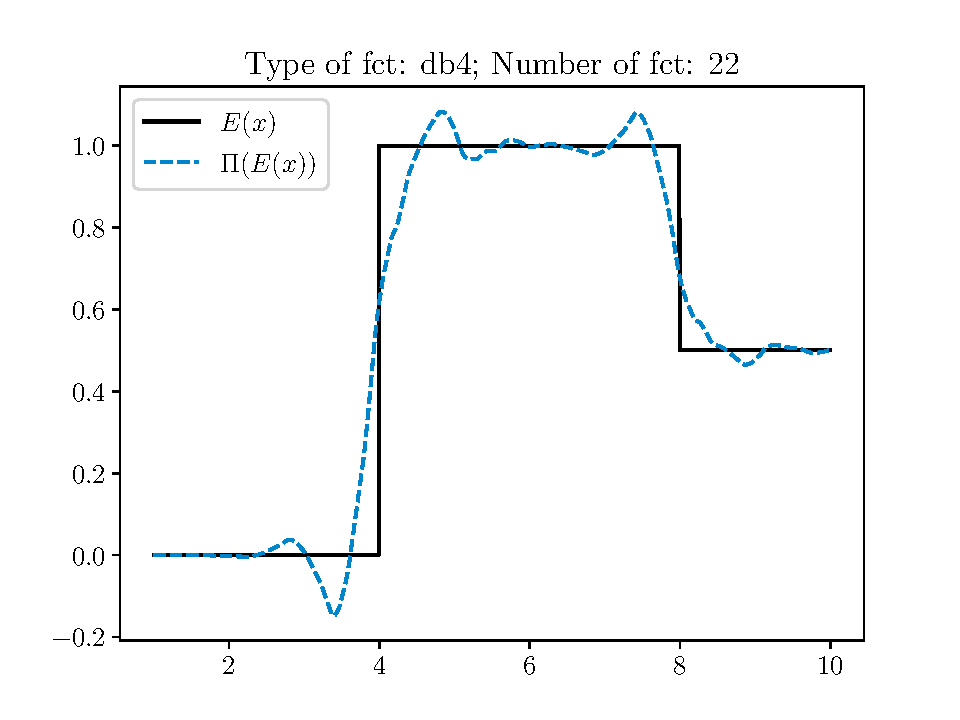
\includegraphics[width=\linewidth]{Figures/db4_N_22_sharp.pdf}
    \caption{Daubechies - sharp function}
\end{subfigure} 
  \begin{subfigure}[t]{0.5\linewidth}
    \centering
    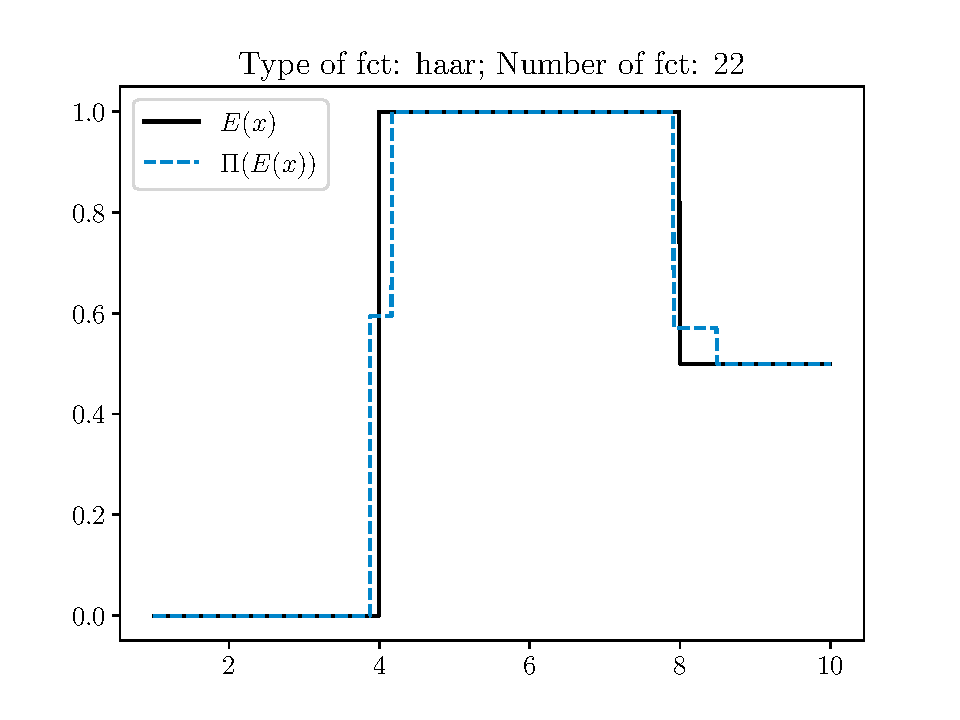
\includegraphics[width=\linewidth]{Figures/haar_N_22_sharp.pdf}
    \caption{Haar - sharp function}
\end{subfigure} 
\caption{Comparison of wavelet truncation for smooth and sharp functions ($1000$ nodes in the function discretisation)}
    \label{Wavelet_1D}
\end{figure}

\subsubsection{Wavelets in 2D}
A two dimensional space distribution has been parametrised with wavelet with the idea of decreasing the number of parameters required to describe it. An illustration of which is given in \cref{Wavelet_2D}.
\begin{figure}[hbpt!]
\begin{subfigure}[t]{0.5\linewidth}
    \centering
    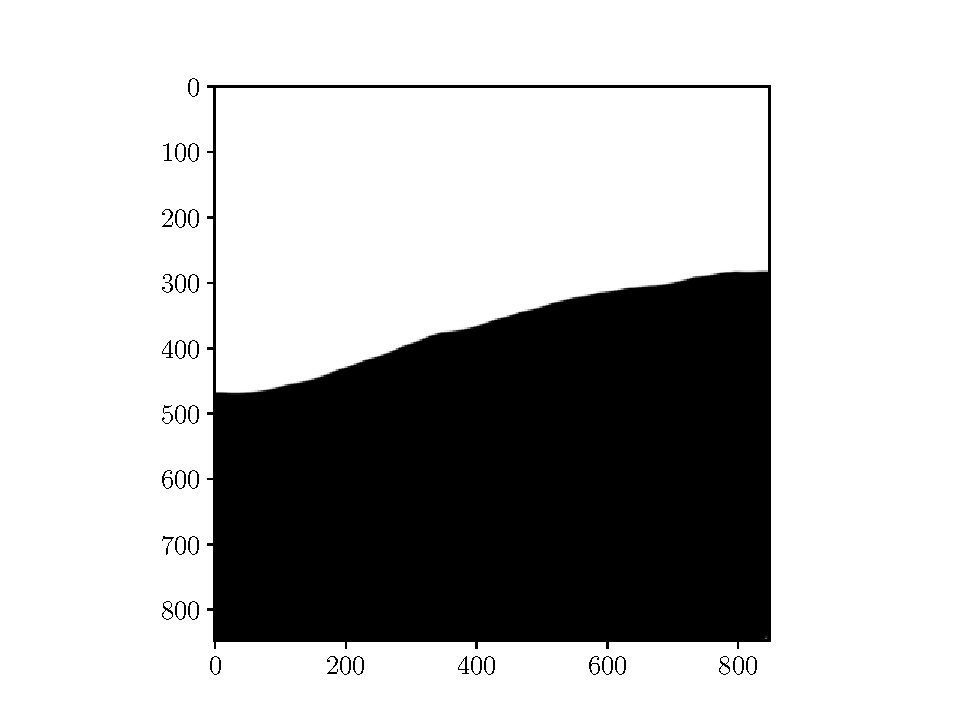
\includegraphics[width=\linewidth]{Figures/2D_ref.pdf}
    \caption{Reference - 720801 parameters}
\end{subfigure}
  \begin{subfigure}[t]{0.5\linewidth}
    \centering
    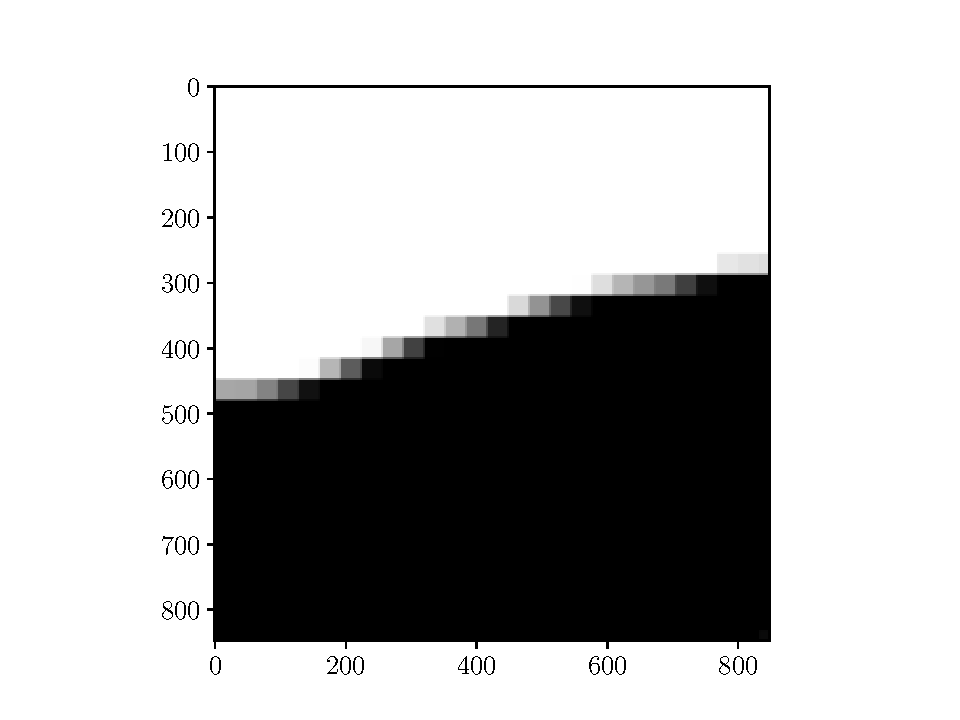
\includegraphics[width=\linewidth]{Figures/2D_comp_haar.pdf}
    \caption{Haar - truncated with 729 parameters}
\end{subfigure}  
\caption{Haar wavelet truncated for sharp 2D discontinuity}
    \label{Wavelet_2D}
\end{figure}

\Rq{\begin{itemize}
    \item Played with the level of wavelet decomposition (fewer parameters per level bu more level) and a fixed number of parameters to keep
    \begin{itemize}
        \item Without relying on the sorting of the value, for sharp discontinuities, we revert to a DG0 interpolation on a coarser mesh.
    \end{itemize}
\end{itemize}}


\subsection{Boundary parametrisation}

If we only care about healthy and diseased zones it seems to be overkill to have several hundreds of parameters to tile the entire space. Using directly a parametrisation of the diseased mobile boundary seems more appropriate. An example of which is illustrated in \cref{fig:space_partition} for two regions in the 1D case.

\begin{figure}
    \centering
    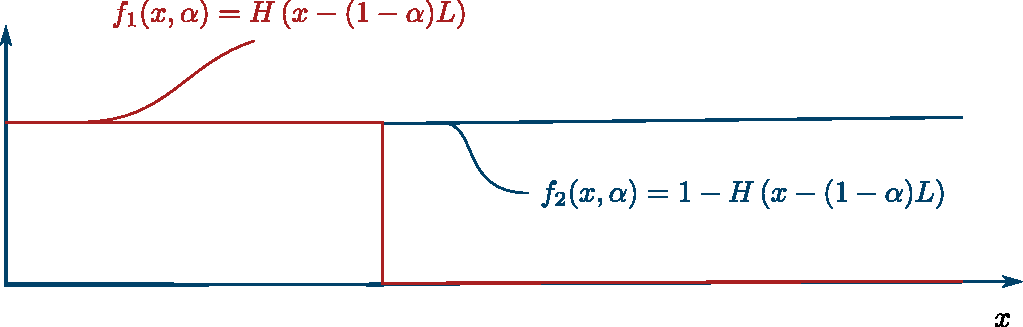
\includegraphics[width = 0.7\linewidth]{Figures/SpacePartition.pdf}
    \caption{Space partition with a mobile boundary}
    \label{fig:space_partition}
\end{figure}

One difficulty that may arise from such an approach is the loss of separability in the TD for the zone parametrisation regarding space. Indeed, the space modes would then depend on those parameters. 

To test the separability assumption, three dummy functions where decomposed using an SVD and then truncated. 

\begin{itemize}
    \item Heaviside \cref{Separability_Heaviside}
    \begin{itemize}
        \item $f(x, \alpha) = H (x-(1-\alpha)L)$
    \end{itemize}
    \item Tanh \cref{Separability_Tanh}
    \begin{itemize}
        \item $f(x, \alpha) =  \text{tanh}(x-(1-\alpha)L)$
    \end{itemize}
    \item Gauss \cref{Separability_Gauss}
    \begin{itemize}
        \item $f(x, \alpha) =  \text{exp}\left( \left(x-(1-\alpha)L\right)^2 \right)$
    \end{itemize}
\end{itemize}

\begin{figure}
\begin{subfigure}[t]{0.5\linewidth}
    \centering
    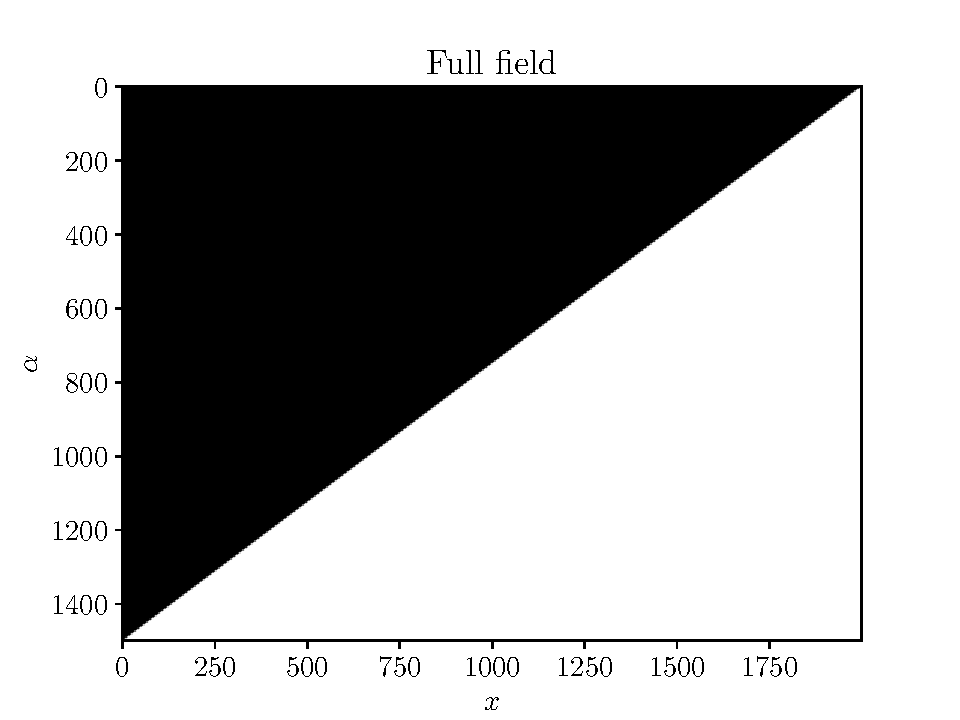
\includegraphics[width=\linewidth]{Figures/FullField_Heaviside.pdf}
    \caption{Full field}
\end{subfigure}
  \begin{subfigure}[t]{0.5\linewidth}
    \centering
    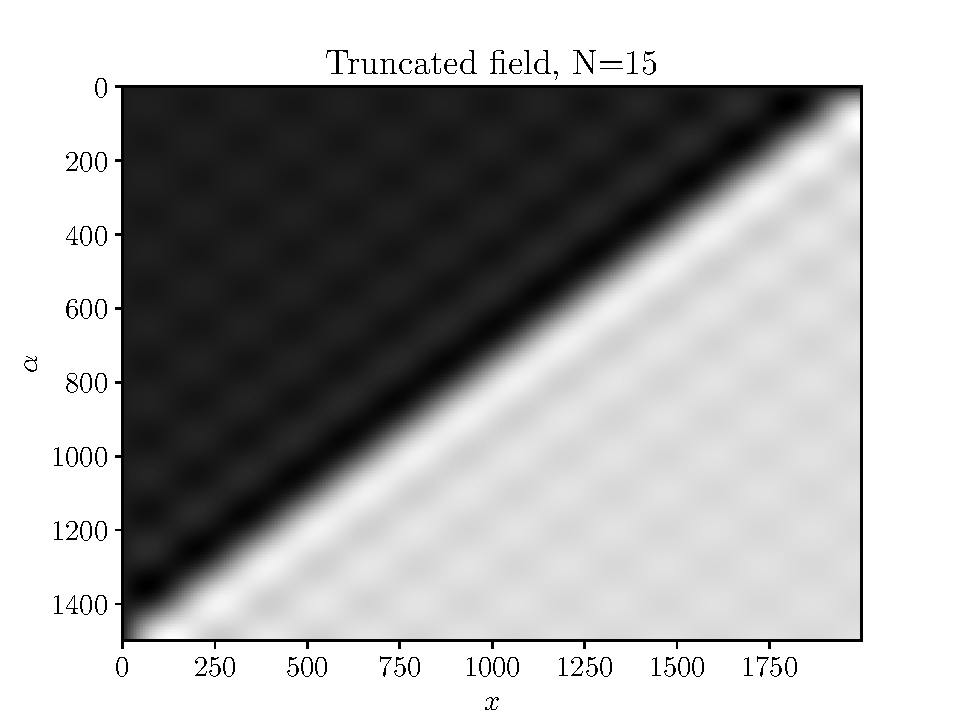
\includegraphics[width=\linewidth]{Figures/TruncatedField_15_Heaviside.pdf}
    \caption{Truncated field}
\end{subfigure}  
  \begin{subfigure}[t]{0.5\linewidth}
    \centering
    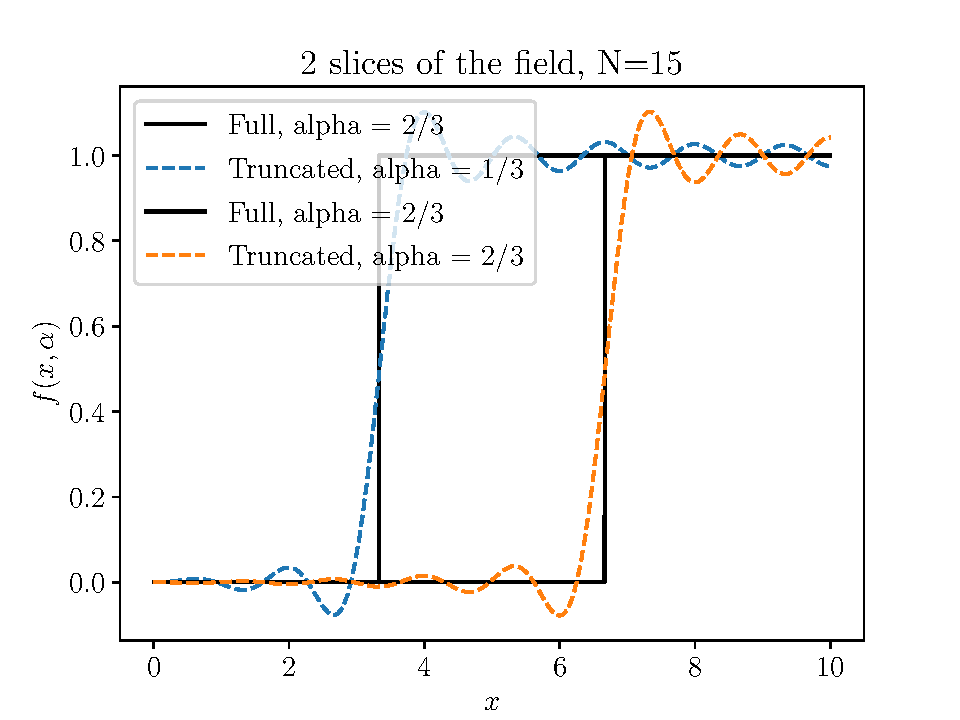
\includegraphics[width=\linewidth]{Figures/Sliced_TruncatedField_15_Heaviside.pdf}
    \caption{Sliced for $\alpha = 1/3$ and $\alpha = 2/3$}
\end{subfigure} 
  \begin{subfigure}[t]{0.5\linewidth}
    \centering
    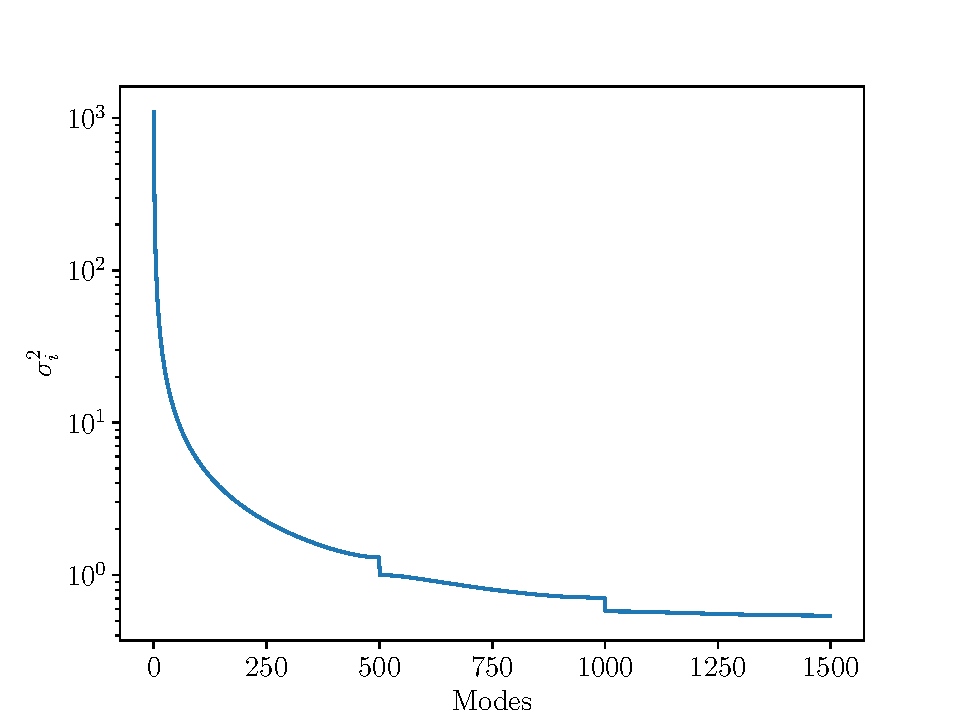
\includegraphics[width=\linewidth]{Figures/SVD_Decay_Heaviside.pdf}
    \caption{SVD decay}
\end{subfigure} 
\caption{Separability study: heaviside}
    \label{Separability_Heaviside}
\end{figure}

\begin{figure}
\begin{subfigure}[t]{0.5\linewidth}
    \centering
    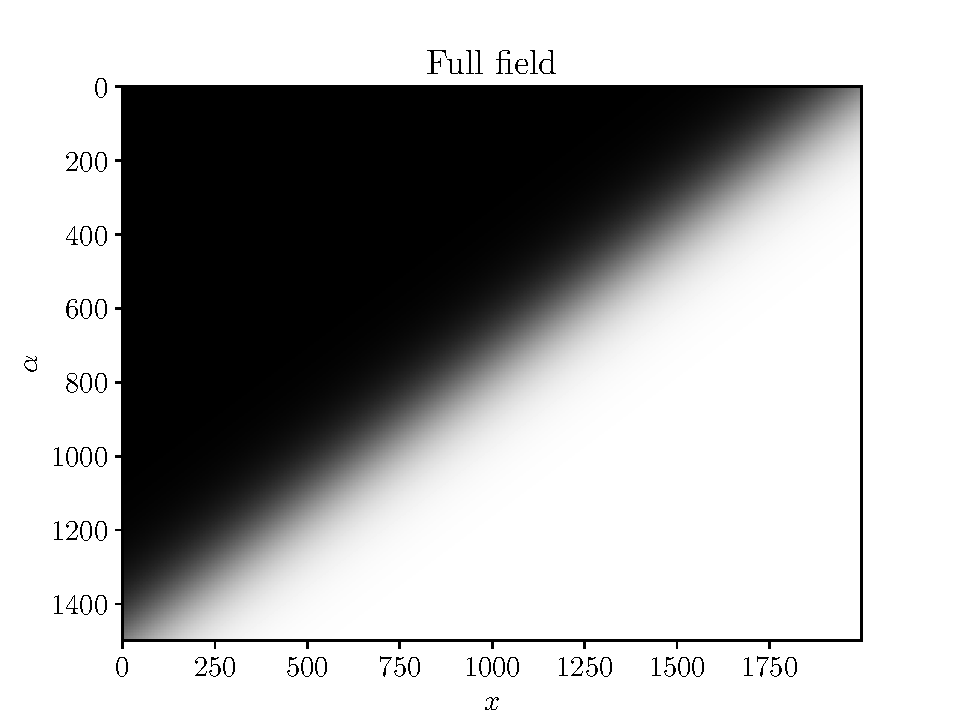
\includegraphics[width=\linewidth]{Figures/FullField_Tanh.pdf}
    \caption{Full field}
\end{subfigure}
  \begin{subfigure}[t]{0.5\linewidth}
    \centering
    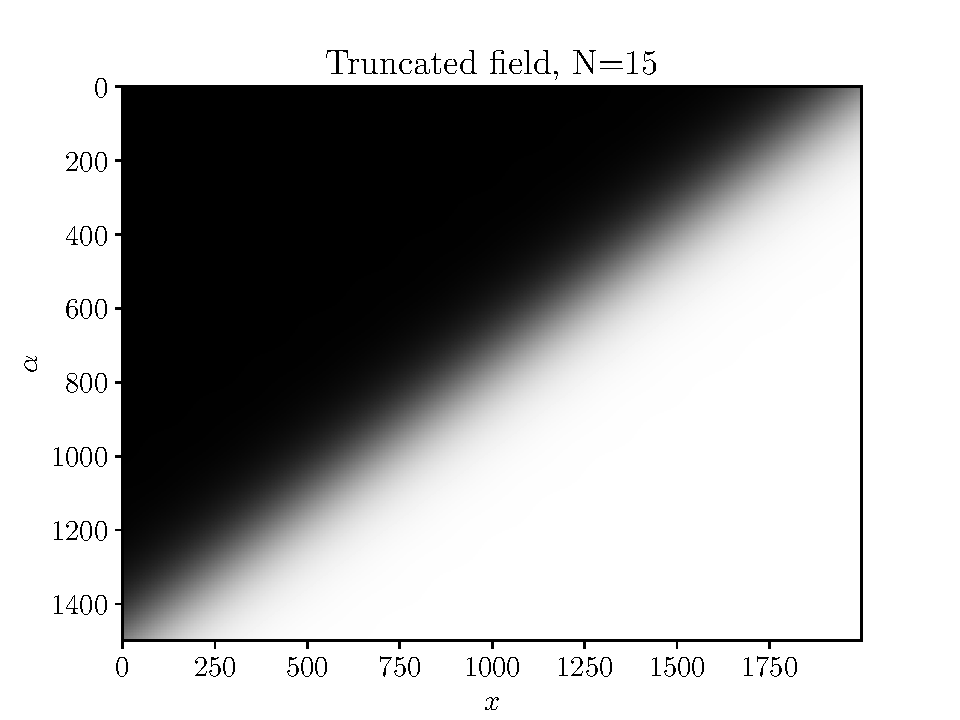
\includegraphics[width=\linewidth]{Figures/TruncatedField_15_Tanh.pdf}
    \caption{Truncated field}
\end{subfigure}  
  \begin{subfigure}[t]{0.5\linewidth}
    \centering
    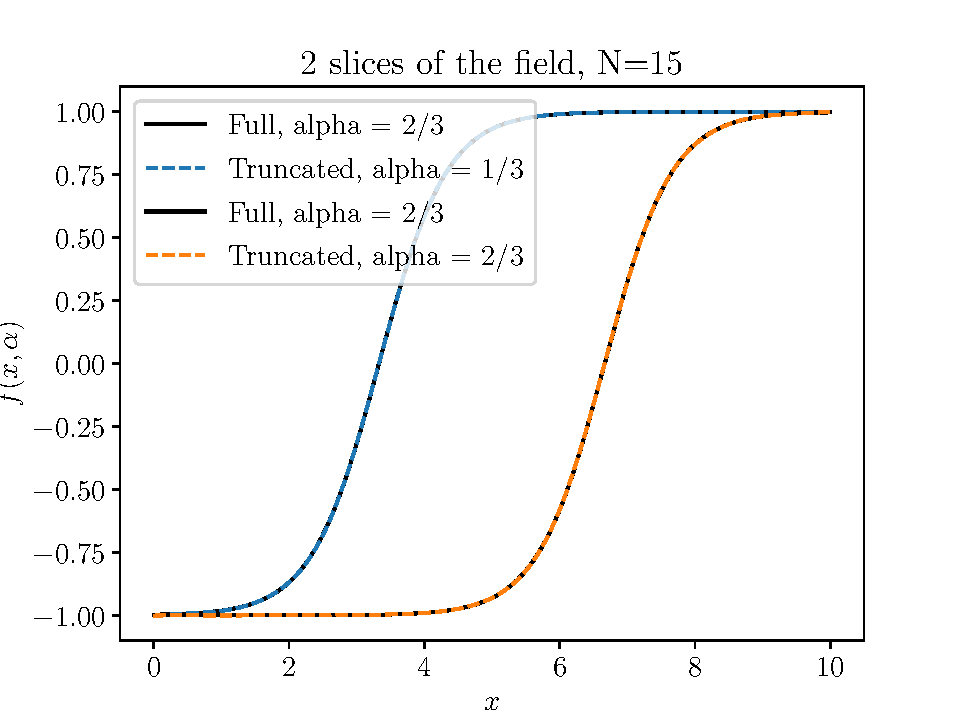
\includegraphics[width=\linewidth]{Figures/Sliced_TruncatedField_15_Tanh.pdf}
    \caption{Sliced for $\alpha = 1/3$ and $\alpha = 2/3$}
\end{subfigure} 
  \begin{subfigure}[t]{0.5\linewidth}
    \centering
    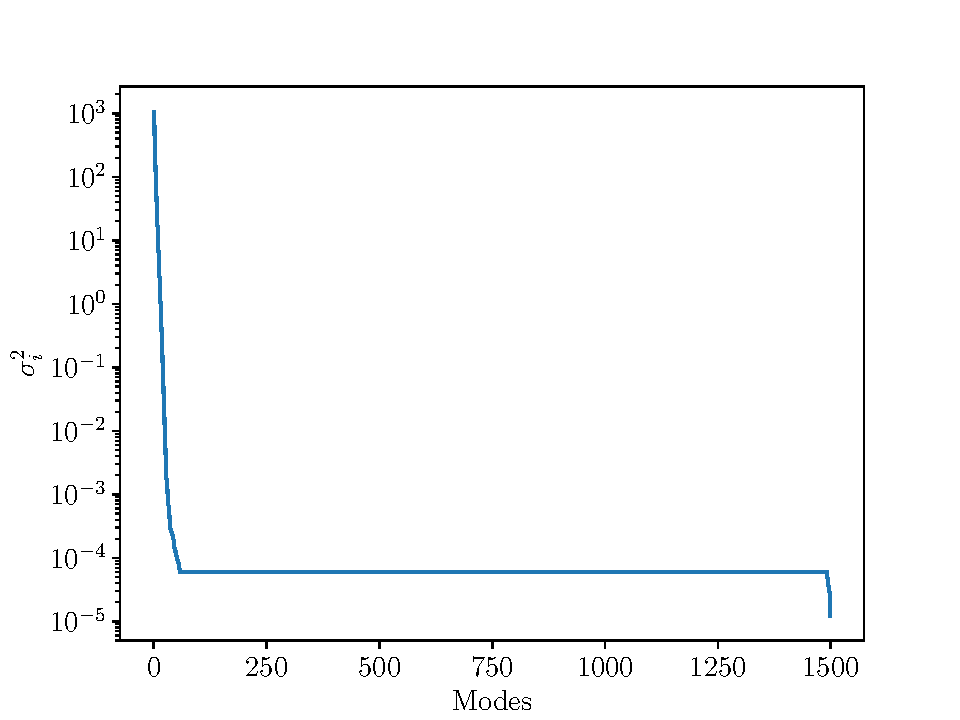
\includegraphics[width=\linewidth]{Figures/SVD_Decay_Tanh.pdf}
    \caption{SVD decay}
\end{subfigure} 
\caption{Separability study: Tanh}
    \label{Separability_Tanh}
\end{figure}

\begin{figure}
\begin{subfigure}[t]{0.5\linewidth}
    \centering
    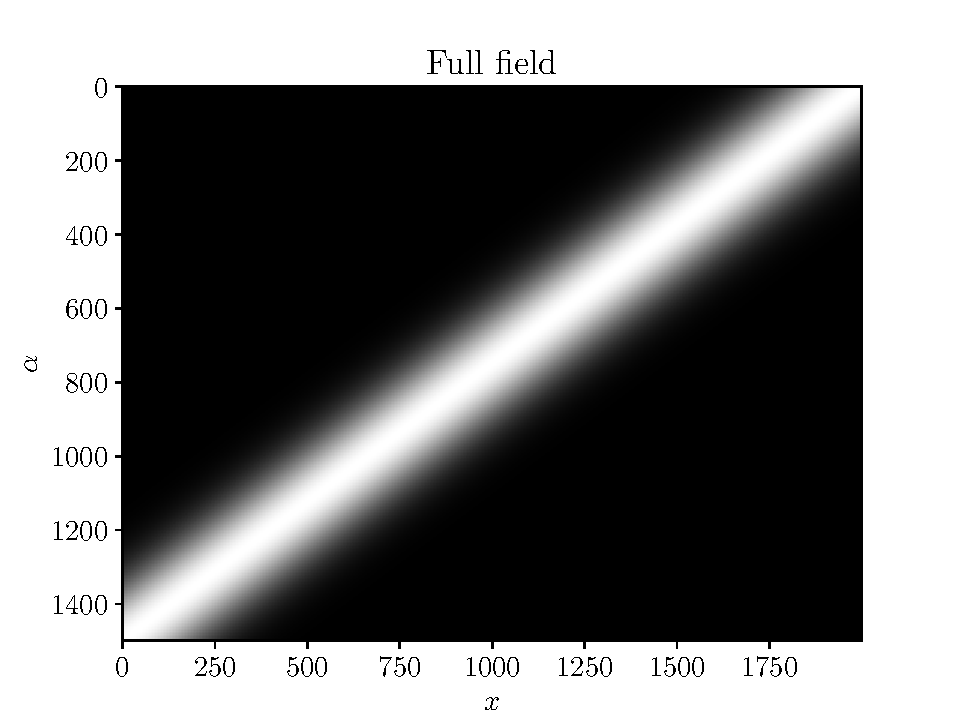
\includegraphics[width=\linewidth]{Figures/FullField_Gauss.pdf}
    \caption{Full field}
\end{subfigure}
  \begin{subfigure}[t]{0.5\linewidth}
    \centering
    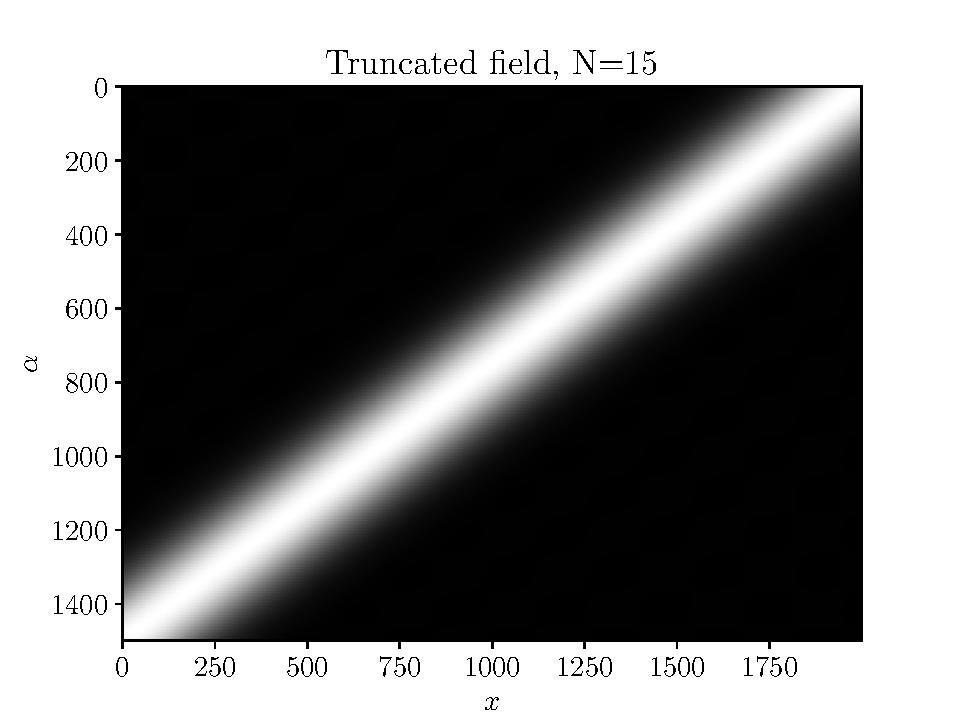
\includegraphics[width=\linewidth]{Figures/TruncatedField_15_Gauss.pdf}
    \caption{Truncated field}
\end{subfigure}  
  \begin{subfigure}[t]{0.5\linewidth}
    \centering
    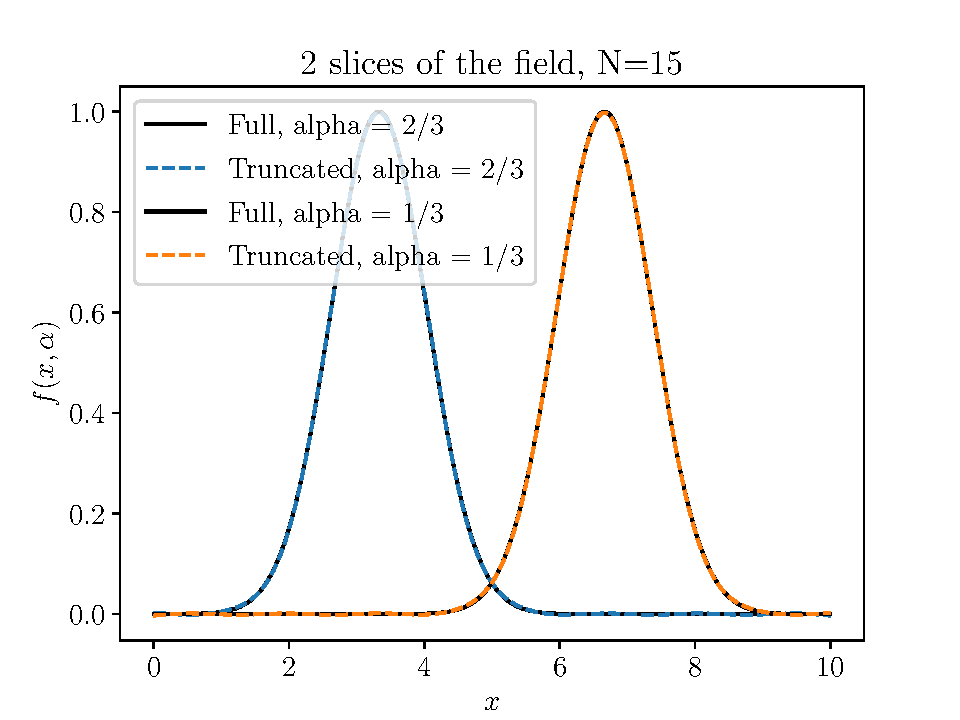
\includegraphics[width=\linewidth]{Figures/Sliced_TruncatedField_15_Gauss.pdf}
    \caption{Sliced for $\alpha = 1/3$ and $\alpha = 2/3$}
\end{subfigure} 
  \begin{subfigure}[t]{0.5\linewidth}
    \centering
    \includegraphics[width=\linewidth]{Figures/SVD_Decay_Gauss.pdf}
    \caption{SVD decay}
\end{subfigure} 
\caption{Separability study: Gauss}
    \label{Separability_Gauss}
\end{figure}

\Rq{Against all odds for smooth functions it is still very much separable. Smoothness should net be a concern as it seems somehow physically sound and natural ?}


\paragraph{\textsc{The Question is:}} Do we want to tile the space or to cluster regions?


If clustering region is fine then a choice of separability for the solution must be made between

    \begin{equation}
        \vect{u}\left(\textcolor{BleuLMS!70}{\vect{x}}, \alpha, \textcolor{LGreenLMS}{\left\{\mu_i\right\}_{i \in \llbracket 1, \beta \rrbracket}}\right) = \sum\limits_{i=1}^m \textcolor{BleuLMS!70}{\overline{\vect{u}}_i(\vect{x})}~\lambda_i^0\left( \alpha \right) ~\textcolor{LGreenLMS}{\prod_{j=1}^{\beta}\lambda_i^j(\mu^j)},
    \end{equation}

    and

    
    \begin{equation}
        \vect{u}\left(\textcolor{BleuLMS!70}{\vect{x}}, \alpha, \textcolor{LGreenLMS}{\left\{\mu_i\right\}_{i \in \llbracket 1, \beta \rrbracket}}\right) = \sum\limits_{i=1}^m \underbrace{\left (\sum\limits_{k=1}^n \lambda_i^{0,k}\left( \alpha \right) \textcolor{BleuLMS!70}{\overline{\vect{u}}_i^k(\vect{x})} \right)}_{\textcolor{BleuLMS!70}{\overline{\vect{u}}_i(\vect{x,\alpha})}} ~\textcolor{LGreenLMS}{\prod_{j=1}^{\beta}\lambda_i^j(\mu^j)}.
    \end{equation}


    Somehow it makes sense to first create the $\textcolor{BleuLMS!70}{\overline{\vect{u}}_i(\vect{x,\alpha})}$ rather than mix the space variability with the parametric variability but it might not be the best solution.

    \Rqs{Intuitively there is a kind of hierarchy in the parameter which I think should be reflected in the decomposition.}{\begin{itemize}
    		\item While wavelets still impose having numerous parameters
    		\begin{itemize}
    			\item Multiplied by the number of modes
    		\end{itemize}
    		\item Here only the number o modes is increased
    		\begin{itemize}
    			\item With the hirearchy in the TD, the number of modes for the other parameters may even be unchanged.
    		\end{itemize}
    \end{itemize}}

\subsubsection{Tensor network, hierarchical tensor decomposition}

There seem to be a large literature on hierarchical tensor decompositions \parencite{bachmayr_tensor_2016} with sparsity results and comparison with the canonical decomposition. Such a hierarchical decomposition relies on multi-linear combination instead of linear interpolations which is a step forward towards non-linear interpolation.
% \subsubsection{Beating Kolmogorov with a nonlinear interpolation ?}
